


 
\documentclass[11pt]{article}
\usepackage[utf8]{inputenc}
\usepackage{mathtools,amsmath,amssymb}
\usepackage{graphicx}
\usepackage{lmodern}
\usepackage[T1]{fontenc}
%\usepackage{microtype}
\usepackage[pagebackref=false]{hyperref}
\usepackage{bbm}
\usepackage{bm}
\usepackage{appendix}
\usepackage{comment}
\numberwithin{equation}{section}
\numberwithin{equation}{subsection}





%\usepackage[textsize=tiny]{todonotes}
 
% \usepackage[notref,notcite]{showkeys}
\usepackage{xspace}
%\usepackage{bibentry}
%\usepackage{easybmat}

\usepackage{graphicx}

\usepackage{subcaption} 

%\usepackage[numbers,sort&compress]{natbib}
%\usepackage{hypernat}
 
\usepackage{tikz}
\usetikzlibrary{decorations.pathreplacing}
% MACROS
% % 
% \newcommand{\cristian}[1]{{\bf (* {\color{ForestGreen}V:{} \small #1}*)}}
% \newcommand{\jorge}[1]{{\bf (* {\color{BlueViolet}G:{} \small #1}*)}}
% \newcommand{\rouven}[1]{{ (* {\color{red}{} \small #1}*)}}
 
\frenchspacing

\newcommand{\changelocaltocdepth}[1]{%
  \addtocontents{toc}{\protect\setcounter{tocdepth}{#1}}%
  \setcounter{tocdepth}{#1}%
}
\newcommand{\id}{I}
\newcommand{\Xt}{\tilde{X}}




\newcommand{\len}{L}
\newcommand{\spe}{N}




\setcounter{tocdepth}{2}

\usepackage[margin=2.5cm]{geometry} 

%%%%%  oscillators
\newcommand{\osc}[1]{\mathbf{#1}}
\newcommand{\oscgreek}[1]{\boldsymbol{#1}}
\newcommand{\dagg}[1]{\bar{#1}}
\newcommand{\ep}{\epsilon}
\newcommand{\ob}{\osc{b}}
\newcommand{\oc}{\osc{c}}
\newcommand{\od}{\osc{d}}
\newcommand{\oab}{\dagg{\osc{a}}}
\newcommand{\obb}{\dagg{\osc{b}}}
\newcommand{\ocb}{\dagg{\osc{c}}}
\newcommand{\odb}{\dagg{\osc{d}}}
\newcommand{\ox}{\oscgreek{\xi}}
\newcommand{\oxb}{\dagg{\oscgreek{\xi}}}
\newcommand{\och}{\oscgreek{\chi}}
\newcommand{\ochb}{\dagg{\oscgreek{\chi}}}
\newcommand{\NN}{\mathbf{N}}
\newcommand{\ccc}{\mathbf{C}}
\newcommand{\qop}{Q}
\newcommand{\sop}{Y}
\newcommand{\q}{\mathbf{\epsilon}}
\newcommand{\ID}{I}
\newcommand{\per}{P}

\newcommand{\EE}{\mathrm{E}}

\newmuskip\pFqmuskip

\newcommand*\pFq[6][8]{%
  \begingroup % only local assignments
  \pFqmuskip=#1mu\relax
  \mathchardef\normalcomma=\mathcode`,
  % make the comma math active
  \mathcode`\,=\string"8000
  % and define it to be \pFqcomma
  \begingroup\lccode`\~=`\,
  \lowercase{\endgroup\let~}\pFqcomma
  % typeset the formula
  {}_{#2}\phi_{#3}{\left[\genfrac..{0pt}{}{#4}{#5};#6\right]}%
  \endgroup
}
\newcommand{\pFqcomma}{{\normalcomma}\mskip\pFqmuskip}


\DeclareMathOperator{\tr}{tr}
\DeclareMathOperator{\Li}{Li}
\DeclareMathOperator{\diag}{diag}


\newcommand{\KL}{\mathcal{K}}
\newcommand{\KR}{\hat{\mathcal{K}}}
\newcommand{\oa}{\mathbf{a}}
\newcommand{\dd}{\mathcal{D}_{\widehat{x}}}
\newcommand{\oad}{\mathbf{a}^{\dagger}}

\newcommand{\phil}{\beta_-}
\newcommand{\phir}{\beta_+}
\newcommand{\ma}{n}

\newcommand{\oaq}{\mathbf{a}_\q}

\newcommand{\oadq}{\mathbf{\bar{a}}_\q}

\newcommand{\N}{\mathbf{N}}
\newcommand{\twoj}{\nu}
\allowdisplaybreaks


\begin{document} 
 
\begingroup
% \centering
\begin{center}
 \begingroup\LARGE
\bf Multispecies stirring process
\par\endgroup
 \vspace{3.5em}
 \begingroup\large \bf
% {Rouven Frassek}
 \par\endgroup
\vspace{2em}

\begingroup\sffamily 
%  
% Università degli Studi di Modena e Reggio Emilia
%University of Modena and Reggio Emilia, 
%\\Department of Physics, Informatics and Mathematics,\\
%Via G. Campi 213/b, 41125 Modena, Italy\\ 
\par\endgroup
\vspace{2em}

 Version: \today
\end{center}
%  

\thispagestyle{empty}

\begin{abstract}
\noindent
...
\end{abstract}

%\vfill 

\tableofcontents

% \newpage

\section{Introduction} 
In the past years duality has been developed to study stochastic processes, especially in the boundary driven case, i.e. when the system is put in contact with boundaries that generate a non-equilibrium current. The literature is huge. We can address , for instance, to \cite{giardina2009duality,carinci2013duality,frassek2020duality}. One application of duality is the attempt to characterize the non equilibrium steady state of boundary driven process via the so called absorption probabilities. Indeed, there are many cases where the dual process has absorbing boundaries. This means that the the chain is eventually empty in the long time scale. Moreover, there are cases in which the steady state of a stochastic process can be computed explicitly, thanks to the integrability property of the system (quantum inverse scattering method, matrix product ansatz). In this direction, some examples can be found in \cite{derrida1993exact,frassek2019non,frassek2020eigenstates}. In the past, the focus has been on processes where one can distinguish, in each site of a certain graph, a (or many) particles or an empty state. However, this particles are indistinguishable, in the sense that you can pile up in a site just one type of particles. Some natural questions arise: what happens if we imagine to assign different colours to the particles? Is the duality property still holding? How far can we push our analysis for the characterization of the non equilibrium steady state?\\
The way one can define a multi-type (or multi-species) interacting particle system is not unique. In the literature there are many. Two of them are the following. On one hand, the \textit{multi-layer models}, in which the process is constructed on a many layer graph where each graph correspond to a type and perform a kind of dynamic (independent jump, exclusion/inclusion walkers) and the layers communicate each other with some "switching probabilities". The state space of the Markov process is the Cartesian product of the state spaces of each layer, i.e. of the two species. For example see \cite{floreani2022switching,redig2022ergodic}. On the other hand, the \textit{single layer models}. Here, there is just one layer, where particles of each type can pile up, in a way that the exclusion dynamic concerns many species together. In other words, now the species can interact "directly", not just by switching layer. Here the state space contains all the species and it is not product anymore. Some examples of such a dynamic can be found in \cite{casini2022uphill,vanicat2017exact,zhou2021orthogonal}. \\
In this work we concentrate our effort in this last "single layer" case with a repulsive process, i.e. a dynamic in which a maximum amount of particles can be present in each site at each time. We will call this amount, the "maximal occupancy" and it will indicated with $\twoj$ where $\twoj\in\mathbb{N}$. Particle of any species can exchange their position in the graph, under this exclusion constraint. The system will be put out of equilibrium and some absorbing duality result are investigated. Moreover, we will use this duality, to study the out of equilibrium steady state. In particular, in case of $\twoj=1$ we should retrieve the model studied in \cite{vanicat2017exact}. We will then exploit this last result and the duality, to write explicitly all the correlations of this \textit{hard-core exclusion} case. The main tool that we will use is the Lie algebraic description of the process, that allows to find the duality as a proper symmetry of the generator. 
\paragraph{Organization of the paper}
\section{The stirring process}
The process studied in this paper is the multi-species stirring process on the geometry of a graph. We consider the general situation where at any time and at any site a mixture of $\nu\in \mathbb{N}$, chosen among $N$ possible species (sometimes called types or colors), is present. Among these $N$ types of particles we will distinguish $N-1$ 'actual' types, labelled with $k\in \{2,\ldots,N\}$ and a 'hole', labelled with $1$. This is an arbitrary choice, indeed one could call any of the $N$ colors the hole. In the description of the dynamic this choice is not important, since one could think about the dynamic as a pure exchange of types between sites, under the constraint that the maximal occupancy at each site is $\nu$. However, studying the duality for the boundary driven case, it will be important to chose an hole type, in order to interpret the dual dynamic as absorbing, i.e. to have, eventually, an empty dual process on the graph. Furthermore, as the configuration of each site at each time is a mixture of $\nu$ particles, one could think about the hole as the only type whose occupation dependes on the occupations of all the true $N-1$ colors. In the two species case, this multi-species stirring process  is the SEP($\nu$) (see \cite{giardina2009duality}, \cite{carinci2013duality}). Indeed one of the two type is the hole (say again $1$) and its dynamics depends on the one of the true type (say 2), under the constaraint that at most $\nu$ type $2$ particles are present at a site at each time. Therefore, the dynamics can be describe only by species $2$. It is interesting to observe that, in case we stop distinguishing the colors of the true particles $\{2,\ldots,N\}$, we retrieve the SEP($\nu$), thus this multi-species stirring process seems its natural generalization. 


\subsection{The infinitesimal generator}
We consider a connected graph $G=(V,\mathcal{E})$ with vertex set $V$ and edge set $\mathcal{E}$.
At each site $x\in V$, we describe the occupation with an $N-$dimensional vector $n^{x}=(n_{1}^{x},\ldots,n_{N}^{x})$ in which the value of the $k$-th component $n_{k}^{x}$ denotes the number of particles of species $k\in \{1,\ldots,N\}$ at site $x\in V$. On each vertex we allow a total  maximal occupancy $\nu\in \mathbb{N}$. Then, the configuration space of the process on the graph $G$ is 
\begin{equation}\label{stateSpace}
    \Omega:=\bigtimes_{x\in V} \Omega_{x}
\end{equation}
where
\begin{equation}
\Omega_{x}:=\left\{(n_{1},\ldots,n_{N})\in\mathbb{N}_0^{N}\;:\; \sum_{k=1}^{N}n_{k}=\twoj\right\}
\end{equation}
We denote a particle configuration as $\mathbf{n}\in \Omega$, where $\mathbf{n}=(n_{k}^{x})_{x\in V,\,k\in\{1,\ldots,N\}}$ .\\
The dynamics consists in an exchange of particles (at Poissonian times) between connected vertices. Moreover, each vertex  exchanges particles with the external environement. The infinitesimal generator of the process reads
\begin{equation}\label{Generator}
    \mathcal{L}=\sum_{(x,y)\in \mathcal{E}}\omega_{x,y}\mathcal{L}_{x,y}+\sum_{x\in V}\Gamma_{x}\mathcal{L}_{x}
\end{equation}
where the quantities $ \omega_{x,y}\geq 0$ are called conductances and $\Gamma_{x}\geq 0$ local inhomogeneities. The generator $\mathcal{L}_{x,y}$ is called the \textit{edge generator}, while $\mathcal{L}_{x}$ is called the \textit{site generator}. These linear operators act on functions $f:\Omega\to \mathbb{R}$ as follows
\begin{equation}\label{edgeGenerator}
\mathcal{L}_{x,y}f(\bm{n})=\sum_{k,\ell=1}^{N}n_{k}^{x}n_{l}^{y}\left[f(\bm{n}-\delta_{x}^{k}+\delta_{\ell}^{x}+\delta_{k}^{y}-\delta_{\ell}^{y})-f(\bm{n})\right]
\end{equation}
\begin{equation}\label{siteGenerator}
    \mathcal{L}_{x}f(\bm{n})=\sum_{k,\ell=1}^{N}\alpha_{k}^{x}n_{\ell}^{x}\left[f(\bm{n}+\delta_{k}^{x}-\delta_{\ell}^{x})-f(\bm{n})\right]
\end{equation}
where 
\begin{equation}
(\delta_{k}^{x})^{y}_{\ell}=\begin{cases}
1\qquad &\text{if}\quad y=x,\;\ell=k\\
0\qquad &\text{otherwise}
\end{cases}
\end{equation}
This means that on the edge $(x,y)\in \mathcal{E}$ at rate $\omega_{x,y}n_{k}^{x}n_{\ell}^{y}$ a particle of type $k$ at site $x$ is exchanged with a particle of tipe $l$ at site $y$; furthermore, on each site $x\in V$ at rate $\Gamma_{x}\alpha_{k}^{x}n_{\ell}^{x}$ a particle of type $\ell$ is replaced with a particle of type $k$. 
See Figure \ref{fig:1}, Figure \ref{fig:2}for a visual description of the dyamics. 
\begin{figure}
    \centering
    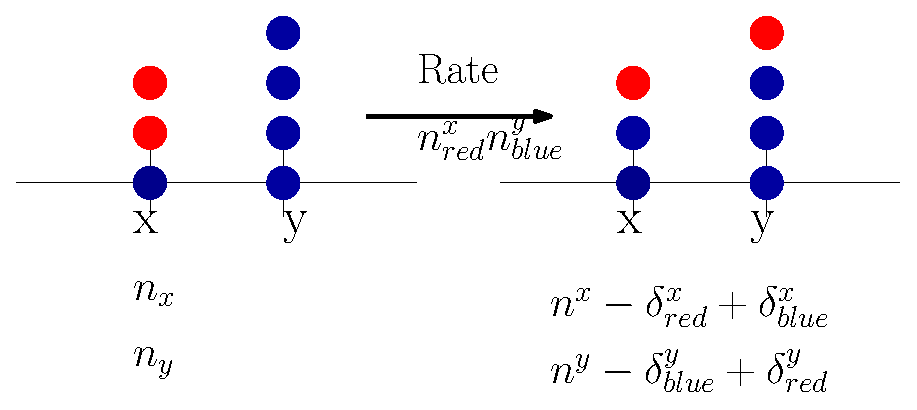
\includegraphics[scale=0.6]{Dyn_stir.eps}
    \caption{The edge dynamics}
    \label{fig:1}
\end{figure}
\begin{figure}
    \centering
    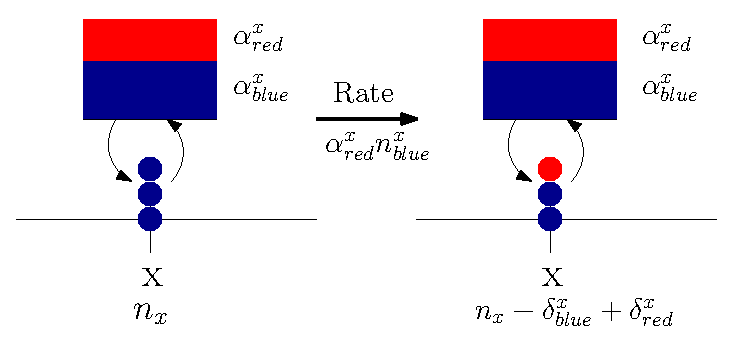
\includegraphics[scale=0.88]{Dyn_stir_bordo.eps}
    \caption{The site dynamics}
    \label{fig:2}
\end{figure}\newline \\
{\color{blue}\textbf{Remark}: 
    We can always assign the name "empty" to one of the species of particles in the above dynamics (let's say, without loss of generality, the species 1). This species would play the role of "compensator" in the exclusion constraint, in the sense that its occupation will always be determined once we know the others, i.e. $\forall x\in V$: 
    \begin{equation}
        n_{1}^{x}=\twoj-\sum_{k=2}^{N}n_{k}^{x}
    \end{equation}
    Moreover, if we set $N=2$ and $\twoj=2j$, we exactly retrieve the SEP(2j), where the empty occupation is indeed $2j-\eta_{x}$ where $\eta_{x}$ is the number of (color blind) particles in the site $x$. In this sense we can think about the stirring process as the natural generalization of the SEP(2j).}
    \begin{flushright}
        $\square$
    \end{flushright}
The process described by the generator \eqref{Generator} is reversible with respect to the homogeneus product measure \begin{equation}\label{reversibleMeasure}
\mu_{rev}=\bigtimes_{x\in V}\mu_{rev}^{x}
\end{equation}
when for any $k\in\{1,\ldots,N\}$
\begin{equation}\label{reversibilityCondition}
\alpha_{k}^{x}=\alpha_{k}\qquad \forall x\in V
\end{equation}
This measure has marginals $\mu_{rev}^{x}$ distributed as 
\begin{equation}
 \mu^{x}_{rev}\sim \text{Multinomial}\left(\twoj,\rho_{1},\ldots,\rho_{N}\right)\quad \text{where}\quad \rho_{k}=\frac{\alpha_{k}}{\sum_{i=1}^{N}\alpha_{i}}
\end{equation}
namely
\begin{equation}
\mu_{rev}^{x}(n^{x})=\frac{\nu!}{\prod_{k=1}^{N}n_{k}^{x}!}\prod_{k=1}^{N}\rho_{k}^{n_{k}^{x}}
\end{equation}
This can be proved just by imposing the detailed balance conditions for the edge and for the site generators. If condition \eqref{reversibilityCondition} is not met, then reversibility is lost: each reservoir at site $x$ wants to fix its own density $\alpha^{x}=(\alpha_{1}^{x},\ldots,\alpha_{N}^{x})$ and currents will arise when at least two of them are different. 
\subsection{The Lie algebraic description}


Consider the Lie algebra $gl(N)$ with generators denoted by $\EE_{ab}$ with $a,b\in \{1,\ldots,N\}$ and commutation relations
\begin{equation}\label{eq:comgl}
\left[\EE_{ab},\EE_{cd}\right]=\EE_{ad}\delta_{bc}-\EE_{cb}\delta_{ad}\qquad \forall a,b\in \{1,\ldots,N\}
\end{equation}
The finite-dimensional representations are labelled by partitions $\lambda=(\lambda_1,\lambda_2,\ldots,\lambda_N)$ of $\nu$ with $\lambda_i\in \mathbb{N}$ and $\sum_{i=1}^N \lambda_i = \nu$. We assume $\lambda_i\geq \lambda_{i+1}$ without loss of generality.
We are interested in the {\em symmetric} finite-dimensional representations with 
\begin{equation}\label{eq:dynkin}
    \lambda=(\twoj,0,\ldots,0) \qquad\text{where}\qquad \twoj\in\mathbb{N}
\end{equation} 
The dimension $M$ of the symmetric representations is given by the combination of $N$ objects in $\twoj$ positions with repetition, namely
\begin{equation}
	M= \frac{(N+\twoj-1)!}{\twoj  !(N-1)!}
\end{equation} 
The basis elements of the vector space $\mathbb{C}^{M}$ are the column vectors 
\begin{equation}
  |n\rangle=  |n_{1},\ldots,n_{N}\rangle,\quad \text{with}\quad n_{i}\in\mathbb{N}_{0}\quad \text{sucht that}\quad \sum_{i=1}^{N}n_{i}=\nu
\end{equation}
%where $\sum_{k=1}^{N}n_{i}=\nu$. 
This basis vector satisfy the orthogonality relation with respect to the Euclidean scalar product 
\begin{equation}\label{ortho}
    \langle m_{1},\ldots,m_{N}|n_{1},\ldots,n_{N}\rangle=\prod_{k=1}^{N}\delta_{m_{k},n_{k}}
\end{equation}
where  $ \langle m_{1},\ldots,m_{N}|$ is the row vector obtained by transposing $|m_{1},\ldots,m_{N}\rangle$ and $\delta_{m_{k},n_{k}}$ is the Kronhecker delta. 
The explicit actions of the algebra generators on the vectors $|n\rangle$ are the following:
\begin{equation}\label{actionE}
	\begin{cases}
		E_{ab}|n_{1},\ldots,n_{a},\ldots,n_{b},\ldots,n_{N}\rangle =n_{b}|n_{1},\ldots,n_{a}+1,\ldots,n_{b}-1,\ldots,n_{N}\rangle\quad a\neq b\\[0.1cm]
		E_{aa}|n_{1},\ldots,n_{a},\ldots,n_{b},\ldots,n_{N}\rangle = n_{a} |n_{1},\ldots,n_{a},\ldots,n_{b},\ldots,n_{N}\rangle\quad a=b
	\end{cases}
\end{equation}  
One can check that the matrices defined in this way satisfy the commutation relations \eqref{eq:comgl} and yield Dynkin weight \eqref{eq:dynkin}.

\noindent
\textbf{Remark}: The symmetric representations $\lambda=(\twoj,0,\ldots,0)$ are dual to the representations $\lambda=(\twoj,\ldots,\twoj,0)$ that can be obtained via 
\begin{equation}
   \bar E_{ab}=\nu\delta_{ab}-E_{N-b+1,N-a+1}
\end{equation}
{\color{red} This needs to be checked and give alternative form of Hamiltonian?}\\
By the Lie algebra above we describe the process with generator \eqref{Generator}. The state space \eqref{stateSpace} is the vector space with basis elements 

%We now define the equivalent of \eqref{stateSpace} in the vector notation
% \begin{equation}
%	\Omega':=\left\{|n\rangle=|n_{1},\ldots,n_{N}\rangle \;:\;n\in\mathbb{N}_0^N,\;\;|n|=\twoj\right\}^{\otimes|V|}
%	\end{equation}
%where we denote 
\begin{equation}
|{\bf n}\rangle=\left(\,\bigotimes_{x\in V}	|n_{1}^{x},\ldots,n_{N}^{x}\rangle\right)
\end{equation}
where we require that $n_{k}^{x}\in \mathbb{N}_{0}$ and $\forall x\in V$ we have $\sum_{k=1}^{N}n_{k}^{x}=\nu$. Sometimes it will bw convenient to write $|n^{x}\rangle$ to denote, for a fixed $x\in V$, the vector $|n_{1}^{x},\ldots,n_{N}^{x}\rangle$. The following orthogonality relation is a consequence of the single site relation \eqref{ortho}
\begin{equation}
    \langle {\bf n}|{\bf m}\rangle =\prod_{x\in V}\prod_{i=1}^N\delta_{n^x_i,m^{x}_i}
\end{equation}
We introduce the Hamiltonian operator

\begin{equation}\label{OriginalHamiltonian}
	\begin{split}
		H=\sum_{x,y\in \mathcal{E}}\omega_{x,y}H_{x,y}+\sum_{x\in V}\Gamma_{x}H_{x}
	\end{split}
\end{equation}
where the edge Hamiltonian is
\begin{equation}\label{edgeHamiltonian}
H_{x,y}=\sum_{k,\ell=1}^{N}\Big(E_{k\ell}^{x} E_{\ell k}^{y}-E_{\ell\ell}^{x} E_{kk}^{y}\Big)
 \end{equation}
  and where the site Hamiltonian is
 \begin{equation}\label{siteHamiltonian}
H_{x}=\sum_{k,\ell=1}^{N}\alpha_{k}^{x}\left(E_{k\ell}^{x}-E_{\ell\ell}^{x}\right)
\end{equation}
Here $E_{kl}^{x}$ is a copy of $E_{kl}$ defined in \eqref{actionE} acting on site $x$. 
Following  \cite{belitsky2015self}, the Hamiltonian and the genertor are linked by
\begin{equation}\label{Hamiltonian-Generator}
H=\mathcal{L}^{T}
\end{equation}
The action of the generator can also be expressed as 
\begin{equation}
    \mathcal{L}f( {\bf n})=\langle f|H| {\bf n}\rangle
\end{equation}
where 
\begin{equation}
    \langle f|=\sum_{ {{\bf n}\in \Omega}}f( {\bf n})\langle  {\bf n}|
\end{equation}

We can write the edge Hamiltonian \eqref{edgeHamiltonian} as a function of the coproduct of the second Casimir of $gl(N)$
\begin{equation}\label{secondCasimir}
    C_{2}=\sum_{a,b=1}^{N}E_{ab}E_{ba}
\end{equation}
that acts diagonally as $C_{2}|\mathbf{n}\rangle=\twoj(\twoj+N)|\mathbf{n}\rangle$ and belogs to the center of $gl(N)$ (i.e. it commutes with all the algebra elements).  
More precisely,  considering the standard coproduct 
\begin{equation}
\begin{split}
\Delta:gl(N)&\to gl(N)\otimes gl(N)\\
E_{ab}&\to E_{ab}\otimes \mathbbm{1}+\mathbbm{1}\otimes E_{ab}
\end{split}
\end{equation}
we have 
\begin{equation}
\Delta(C_{2})=\sum_{a,b=1}^{N}\Delta(E_{ab})\Delta(E_{ba})=2\sum_{a,b=1}^{N}E_{ab}\otimes E_{ba}+C_{2}\otimes \mathbbm{1}+\mathbbm{1}\otimes C_{2}
\end{equation}
Then, one can check that 
\begin{equation}\label{hamiltonianCasimir}
	H_{x,y}=\frac{1}{2}\Delta^{x,y}(C_{2})-\twoj(2\twoj+N)
\end{equation}
where $\Delta^{x,y}(C_2)$ denotes a copy of $\Delta(C_2)$ acting on  
the edge $(x,y)\in \mathcal{E}$.


\begin{comment}
We introduce the Hamiltonian operator

\begin{equation}\label{OriginalHamiltonian}
	\begin{split}
		H=\sum_{x,y\in \mathcal{E}}\omega_{x,y}H_{x,y}+\sum_{x\in V}\Gamma_{x}H_{x}
	\end{split}
\end{equation}
where the edge Hamiltonian is
\begin{equation}\label{edgeHamiltonian}
H_{x,y}=\sum_{k,l=1}^{N}E_{kl}^{x}\otimes E_{lk}^{y}-E_{ll}^{x}\otimes E_{kk}^{y}
 \end{equation}
 and where the site Hamiltonian is
 \begin{equation}\label{siteHamiltonian}
H_{x}=\sum_{k,l=1}^{N}\alpha_{k}^{x}\left(E_{kl}^{x}-E_{ll}^{x}\right)
\end{equation}
Here $E_{kl}^{x}$ is a copy of $E_{kl}$ defined in \eqref{actionE} acting on site $x$. 

We can write this Hamiltonian in function of the coproduct of the second Casimir
\begin{equation}
    C_{2}=\sum_{a,b=1}^{N}E_{ab}E_{ba}
\end{equation}
It reads
\begin{equation}
	H_{x,y}=\left\{\frac{1}{2}\Delta^{xy}(C_{2})-\twoj(2\twoj+N)\frac{1}{2}\mathbbm{1}^{x}\otimes\mathbbm{1}^{y}\right\}
\end{equation}
Here we introduced the standard coproduct
\begin{equation}
\begin{split}
\Delta:gl(N)&\to gl(N)\otimes gl(N)\\
E_{ab}&\to E_{ab}\otimes \mathbbm{1}+\mathbbm{1}\otimes E_{ab}
\end{split}
\end{equation} acting on sites $x,y$ and used that $C_{2}|n\rangle=\twoj(\twoj+N)|n\rangle$. 
\end{comment}
 



\section{Duality}\label{sectionDuality}
\subsection{Definition}
Consider two Markov processes $(\eta_{t})_{t\geq 0}$ defined on a state space $\Omega$ and $(\xi_{t})_{t\geq 0}$ defined on a state space $\widetilde{\Omega}$. We say that they are dual, with respect to a duality function $D:\Omega\times \widetilde{\Omega}\to \mathbb{R}$, if $\forall \eta\in\Omega$, $\forall \xi\in\widetilde{\Omega}$ and $\forall t> 0$ we have 
\begin{equation}
    \mathbb{E}_{\eta}\left[D(\eta_{t},\xi)\right]=\mathbb{E}_{\xi}\left[D(\eta,\xi_{t})\right]
\end{equation}
where $\mathbb{E}_{\eta}$ denotes the expectation with respect the law of the Markov process $(\eta_{t})_{t\geq 0}$ initialized with the particle configuration $\eta$, whereas $\mathbb{E}_{\xi}$ denotes the expectation with respect to the law of the Markov process $(\xi_{t})_{t\geq 0}$ initialized with the particle configuration $\xi$.
The duality definition can also be formulated as a relation between the generators. Call $\mathcal{L}$ the generator of $(\eta_{t})_{t\geq0}$ and $\widetilde{\mathcal{L}}$ the generator of $(\xi_{t})_{t\geq 0}$, then we say that these two processes are dual with respect to the duality function $D:\Omega\times \widetilde{\Omega}\to \mathbb{R}$ if $\forall \eta\in\Omega$ and $\forall \xi\in\widetilde{\Omega}$
\begin{equation}\label{dualityRelationGenerator}
    \left(\mathcal{L}D(\cdot,\xi)\right)(\eta)=\left(\widetilde{\mathcal{L}}D(\eta,\cdot)\right)(\xi)
\end{equation}
In the specific case where $\mathcal{L}=\widetilde{\mathcal{L}}$ we say that the process is self-dual.
\newline
\newline
\textbf{Remark}:
when the state spaces of the dual processes is finite, the generators and the duality function are matrices with elements $\mathcal{L}(\eta,\eta^{'})$, $\widetilde{\mathcal{L}}(\xi,\xi^{'})$ and $D(\eta,\xi)$ for arbitrary $\eta,\eta^{'}\in\Omega$ and $\xi,\xi^{'}\in \widetilde{\Omega}$. Therefore, we can write the duality relation \eqref{dualityRelationGenerator} as 
\begin{equation}
    \sum_{\eta^{'}\in\,\Omega}\mathcal{L}(\eta,\eta^{'})D(\eta^{'},\xi)=\sum_{\xi^{'}\in\, \widetilde{\Omega}}\widetilde{\mathcal{L}}(\xi,\xi^{'})D(\eta,\xi^{'})
\end{equation}
that can be read as
\begin{equation}\label{dualityIntertwines}
    \mathcal{L}D=D\widetilde{\mathcal{L}}^{\,T}
\end{equation}
where the superscript $T$ denotes the matrix transposition. Therefore, the duality relation \eqref{dualityIntertwines} is an intertwining between two linear operators $\mathcal{L}$ and $\widetilde{\mathcal{L}}$. Working with the Hamiltonian operators the duality relation \eqref{dualityIntertwines} reads 
\begin{equation}\label{DualityRelation}
    H^{T}D=D\widetilde{H}
\end{equation}
\subsection{Duality for the multi-species stirring process}\label{statementDualitySubsection}
In this section we show that the process $(\mathbf{n}(t))_{t\geq 0}$, defined by the generator \eqref{Generator}, is dual to a process $(\bm{\xi}(t))_{t\geq 0}$ taking values in the enlarged state space
\begin{equation}\label{dualStateSpace}
    \widetilde{\Omega}= \bigtimes_{x\in V} \widetilde{\Omega}_{x}\ = \bigtimes_{x\in V} (\Omega_{x}\times \mathbb{N}_{0}^{N-1})
\end{equation}
To each site $x\in V$ we associate an ``extra site'', denoted $\widehat{x}$,
where dual particles will accumulate in the course of time. 
We write the configurations $\bm{\xi} \in \widetilde\Omega$  as
\begin{equation}
    \bm{\xi}=\left(r_{1}^{x},\ldots,r_{N}^{x},m_{2}^{\widehat{x}},\ldots,m_{N}^{\widehat{x}}\right)_{x\in V}
\end{equation}
where the component $r_{k}^{x}$ is interpreted as the number of dual particles of type $k\in \{1,\ldots,N\}$ at site $x$, 
and the component $m_{k}^{\widehat{x}}$  gives the number of dual particles of type $k\in \{2,\ldots,N\}$ at 
the extra-site $\widehat{x}$ connected to $x\in V$.
 The  generator of the dual process is 
 \begin{equation}\label{DualGenerator}
    \widetilde{\mathcal{L}}=\sum_{(x,y)\in \mathcal{E}}\omega_{x,y}\mathcal{L}_{x,y}+\sum_{x\in V}\Gamma_{x}\widetilde{\mathcal{L}}_{x}
\end{equation}
where 
$\mathcal{L}_{x,y}$ is defined in \eqref{siteGenerator} and, for any function $f:\widetilde{\Omega}\to \mathbb{R}$ 
\begin{equation}\label{siteDualGenerator}
    \widetilde{\mathcal{L}}_{x}f(\bm{\xi})=\sum_{i=1}^{N}\alpha_{i}^{x}\sum_{k=2}^{N}r_{k}^{x}\left(f(\bm{\xi}-\delta_{k}^{x}+\delta_{1}^{x}+\delta_{k}^{\widehat{x}})-f(\bm{\xi})\right)
\end{equation}
and the duality function is 
\begin{equation}\label{dualityElements}
	D(\bm{n},\bm{\xi})=\prod_{x\in V}\left(\frac{(2j-\sum_{k=2}^{N}r_{k}^{x})!}{\nu!}\prod_{k=2}^{N}\frac{n_{k}^{x}!}{(n_{k}^{x}-r_{k}^{x})!}\left(\rho_{k}^{x}\right)^{m_{k}^{\widehat{x}}}\,\right)
\end{equation}
where we denote the \textit{density} of the species $k\in \{2,\ldots,N\}$ at the reservoir connected with the site $x\in V$  by 
\begin{equation}
\rho_{k}^{x}:=\frac{\alpha_{k}^{x}}{\sum_{i=1}^{N}\alpha_{i}^{x}}
\end{equation}
\newline
On one hand, the edge part of the dual generator \eqref{DualGenerator} is a copy of \eqref{edgeGenerator}, therefore it performs the stirring dynamics on the graph. On the other hand, the dual generator \eqref{siteDualGenerator} replaces a particle of any type $k\in\{2,\ldots,N\}$ at site $x$ with a particle of type $1$ and creates a particle of the same type $k$ at the extra-site $\widehat{x}$. This last transition is performed with rate $\sum_{i=1}^{N}\alpha_{i}^{x}r_{k}^{x}$. This means that eventually the dual process voids the graph, putting all the dual particles of species $\{2,\ldots,N\}$ in the extra-sites. In other words the extra-sites play the role of absorbing boundaries. 
\newline \newline
\textbf{Remark}: in the reversible situation, i.e. when $\forall x\in V$ $\alpha_{k}^{x}=\alpha_{k}$, the expectation  of the duality function  $D(\bm{n},\bm{\xi})$ with   $\bm{n}$ distributed as  $\mu_{rev} = \bigtimes_{x\in V}\text{Multinomial}\left(\twoj, p_{1},\ldots,p_{N}\right)$ is
\begin{equation}
\mathbb{E}_{\mu^{rev}}\left[D(\bm{n},\bm{\xi})\right]=\prod_{k=2}^{N}\left(\rho_{k}^{x}\right)^{\sum_{x\in V}r_{k}^{x}+\sum_{x\in V}m_{k}^{\widehat{x}}}\qquad \forall \bm{n}\in \Omega,\quad\forall \bm{\xi}\in \widetilde{\Omega}
\end{equation}

\subsection{Proof of duality}
To prove duality between $(\bm{n}(t))_{t\geq 0}$ and $(\bm{\xi}(t))_{t\geq 0}$ we  show that \eqref{dualityIntertwines} is fulfilled.  To show this, we will use the Hamiltonians (linked with the generators by \eqref{Hamiltonian-Generator}) and their Lie algebraic description. Indeed, in this formalism the proof reduces in finding symmetries and exponential transformation of generators of the Lie algebra.\\
The configuration space  \eqref{dualStateSpace} of the dual process is the collection of vectors
\begin{equation}
    |\bm{\xi}\rangle=\bigotimes_{x\in V}\left(|r_{1}^{x},\ldots,r_{N}^{x}\rangle\otimes |m_{2}^{\widehat{x}},\ldots,m_{N}^{\widehat{x}}\rangle\right)
\end{equation}
The Hamiltonian of the dual process reads as
\begin{equation}\label{DualHamiltonian}
    \widetilde{H}=\sum_{x,y\in \mathcal{E}}\omega_{x,y}H_{x,y}+\sum_{x\in V}\Gamma_{x}\widetilde{H}_{x}
\end{equation}
where $H_{x,y}$ is the one defined in \eqref{edgeHamiltonian}, while 
\begin{equation}\label{siteDualHamiltonian}
    \widetilde{H}_{x}=\sum_{i=1}^{N}\alpha_{i}^{x}\sum_{k=2}^{N}\left((a^{\dagger})_{k}^{\widehat{x}}\,E_{1k}^{x}-E_{kk}^{x}\right)
\end{equation}
Here we introduced bosonic creation operator $a^{\dagger}$ acting as $a^{\dagger}|q\rangle=|q+1\rangle$ on a generic vector $|q\rangle$ with $q\in \mathbb{N}_{0}$, so that in \eqref{siteDualHamiltonian} 
$(a^{\dagger})_{k}^{\widehat{x}}$ denotes a copy of $a^{\dagger}$ acting on the extra-site $\widehat{x}$ and on the species $k\in\{2,\ldots,N\}$. \\
The Hamiltonians \eqref{OriginalHamiltonian} and \eqref{DualHamiltonian} are dual in the sense of \eqref{DualityRelation} with respect to the duality matrix $D$ defined as 
\begin{equation}\label{dualityMatrix}
    D=\prod_{x\in V}d_{x}\otimes \dd
\end{equation}
where
\begin{equation}
d_{x}=R_{x}\exp{(E^{x})}
\end{equation}
with 
\begin{equation}\label{EquationEx}
E^{x}=\sum_{a=2}^{N}E_{a1}^{x}
\end{equation}
and
\begin{equation}\label{Rmatrix}
    R_{x}=\sum_{n^{x}\in\Omega_{x}}\frac{\prod_{k=1}^{N}n_{k}^{x}}{\nu!}|n_{1}^{x},\ldots,n_{N}^{x}\rangle\langle n_{1}^{x},\ldots,n_{N}^{x}|
\end{equation}
and where 
\begin{equation}\label{dualityMatrix2}
\dd=\sum_{m_{2}^{\widehat{x}},\ldots,m_{N}^{\widehat{x}}=0}^{\infty}\prod_{k=2}^{N}\left(\rho_{k}^{x}\right)^{m_{k}^{\widehat{x}}}\langle m_{2}^{\widehat{x}},\ldots,m_{N}^{\widehat{x}}|
\end{equation}
The matrix $R_{x}$ is diagonal. Its elements are related to the inverse of the weights of the reversible measure \eqref{reversibleMeasure}. In particular, to obtain these elements, we have considered the weights of \eqref{reversibleMeasure} when all the parameters $p_{i}=\frac{1}{N}$. Then, the constant $\left(\frac{1}{N}\right)^{\nu}$ has been neglected, since it does not change the duality relation. This $R_{x}$ is called the ``cheap'' duality matrix (see \cite{giardina2009duality}). \\
Since \eqref{dualityMatrix} is product over sites, \eqref{DualityRelation} is equivalent to proving that 
\begin{equation}\label{edgeDualRealtion}
    H_{x,y}^{T}D=DH_{x,y}\qquad \forall (x,y)\in \mathcal{E}
\end{equation}
and 
\begin{equation}\label{siteDualRelation}
    H_{x}^{T}D=D\widetilde{H}_{x}\qquad \forall x\in V.
\end{equation}
We perform the proof in three steps: first we will show that matrix \eqref{dualityMatrix} has elements \eqref{dualityElements}; second we will prove \eqref{edgeDualRealtion}; finally we will show\eqref{siteDualRelation}. 
\paragraph{Elements of the duality matrix.}We aim to show that 
\begin{equation}\label{proofDualityElements}
\langle \bm{n}|D|\bm{\xi}\rangle=D(\bm{n},\bm{\xi})\qquad   \forall \bm{n}\in \Omega,\quad \bm{\xi}\in \widetilde{\Omega}
\end{equation}
with $D(\bm{n},\bm{\xi})$ defined in \eqref{dualityElements}. 
Fix an arbitrary site $x\in V$
\begin{align*}
	 &\langle n^{x}|d_{x}\otimes \dd|\xi^{x}\rangle\\&=\langle n_{1}^{x},\ldots,n_{N}^{x}| (\exp{(E_{12}^{x}+\ldots+E_{1N}^{x}}))^{T}R_{x}\otimes\sum_{m_{2}^{\widehat{x}},\ldots,m_{N}^{\widehat{x}}=0}^{\infty}\prod_{k=2}^{N}\left(\rho_{k}^{x}\right)^{m_{k}^{\widehat{x}}}\langle m_{2}^{\widehat{x}},\ldots,m_{N}^{\widehat{x}}|
	 \\&|r_{1}^{x},\ldots,r_{N}^{x}\rangle_{x} \otimes |q_{2}^{\widehat{x}},\ldots,q_{N}^{\widehat{x}}\rangle
\end{align*}
On one hand, on the extra-site $\widehat{x}$ we have 
\begin{align*}
\sum_{m_{2}^{\widehat{x}},\ldots,m_{N}^{\widehat{x}}=0}^{\infty}\prod_{k=2}^{N}\left(\rho_{k}^{x}\right)^{m_{k}^{\widehat{x}}}\langle m_{2}^{\widehat{x}},\ldots,m_{N}^{\widehat{x}}||q_{2}^{\widehat{x}},\ldots,q_{N}^{\widehat{x}}\rangle=\prod_{k=2}^{N}\left(\rho_{k}^{x}\right)^{m_{k}^{\widehat{x}}}
\end{align*}
where we used the orthogonality relation \eqref{ortho}. 
On the other hand, on the site $x$, we have 
\begin{align*}
&\langle n_{1}^{x},\ldots,n_{N}^{x}|(\exp{(E_{12}^{x}+\ldots+E_{1N}^{x})})^{T}R_{x}|r_{1}^{x},\ldots,r_{N}^{x}\rangle\\&= \langle  n_{1}^{x},\ldots,n_{N}^{x}|\left(\sum_{k_{2}=0}^{\infty}\frac{\left\{\left(E_{12}^{x}\right)^{T}\right\}^{k_{2}}}{k_{2}!}\ldots\sum_{k_{N}=0}^{\infty}\frac{\left\{\left(E_{1N}^{x}\right)^{T}\right\}^{k_{N}}}{k_{N}!}\sum_{s\in\chi}\frac{s_{1}^{x}!\ldots s_{N}^{x}!}{\nu!}|s_{1}^{x},\ldots,s_{N}^{x}\rangle\langle s_{1}^{x},\ldots,s_{N}^{x}|\right)|r_{1}^{x},\ldots,r_{N}^{x}\rangle\\&=
\sum_{k_{2}=0}^{n_{1}^{x}}\ldots\sum_{k_{N}=0}^{n_{N}^{x}}\langle n_{1}^{x}+k_{2}+\ldots+k_{N},n_{2}^{x}-k_{2},\ldots,n_{N}^{x}-k_{N}|_{x}\frac{n_{2}^{x}!\ldots n_{N}^{x}!}{(n_{2}^{x}-k_{2})!\ldots(n_{N}^{x}-k_{N})!}
\\&\cdot 
\frac{1}{k_{2}!,\ldots,k_{N}!}\frac{r_{1}^{x}!\ldots r_{N}^{x}!}{\nu!}|r_{1},\ldots,r_{N}\rangle_{x}\\&=
\frac{(2j-\sum_{k=2}^{N}r_{k}^{x})}{\nu!}\prod_{k=2}^{N}\frac{n_{k}^{x}!}{(n_{k}^{x}-r_{k}^{x})!}
\end{align*}
where in the last equality we applied the orthogonality relations \eqref{ortho} and the fact that $r_{1}^{x}=\nu-\sum_{k=2}^{N}r_{k}^{x}$. Finally, by taking the product over $x\in V$ \eqref{proofDualityElements} is proved.
\begin{flushright}
    $\square$
\end{flushright}
\paragraph{Proof of \eqref{edgeDualRealtion}.}To show \eqref{edgeDualRealtion} we need two 'ingredients'. First the existence of a similarity transformation between the Hamiltonian $H_{x,y}$ defined in \eqref{edgeHamiltonian} and its transposed. As we will show, this similarity transformation is $R_{x}$ defined in \eqref{Rmatrix}. Second, the possibility of finding a symmetry for the Hamiltonian \eqref{edgeHamiltonian}. Exploiting the fact that $H_{x,y}$ is a linear function of the coproduct of the second Casimir of $gl(N)$, (see \eqref{hamiltonianCasimir}) this symmetry is $\exp{(E^{x})}\exp{(E^{y})}$ with $E^{x}$ defined in \eqref{EquationEx}. \\
We show that 
\begin{equation}\label{transpositionPropertyR}
(E_{ab}^{x})^{T}=R_{x}E_{ab}^{x}R_{x}^{-1}\qquad \forall x\in V
\end{equation}
Indeed
\begin{align*}
R_{x}E_{ab}^{x}R_{x}^{-1}=&\sum_{r^{x}\in\Omega_{x}}\left(\frac{r_{1}^{x}!\ldots r_{N}!}{\nu!}|r_{1}^{x},\ldots,r_{N}^{x}\rangle \langle r_{1}^{x},\ldots, r_{N}^{x}|\right)
	\\&
	\sum_{s^{x}\in \Omega_{x},}\left(s_{b}^{x}|s_{1}^{x},\ldots,s_{a}^{x}+1,\ldots,s_{b}^{x}-1,\ldots s_{N}^{x}\rangle \langle s_{1}^{x},\ldots,s_{N}^{x}|\right)
	\\&
	\sum_{n_{x}\in\Omega_{x}}\left(\frac{\nu!}{n_{1}!\ldots n_{N}!}|n_{1}^{x},\ldots,n_{N}^{x}\rangle \langle n_{1}^{x},\ldots, n_{N}^{x}|\right)
 \\=&\sum_{r^{x}\in \Omega_{x}}
	r_{a}^{x}|r_{1}^{x},\ldots,r_{N}^{x}\rangle \langle r_{1}^{x},\ldots,r_{a}^{x}-1,\ldots,r_{b}^{x}-1,\ldots,r_{N}^{x}|
	\\=&
	\left(E_{ba}^{x}\right)^{T}
\end{align*}
where in the up to last equation we used the orthogonality relation \eqref{ortho}. 
Equation \eqref{transpositionPropertyR} implies that 
\begin{equation}\label{transpositionPropertyH}
    H_{x,y}^{T}=\left(R_{x}R_{y}\right)H_{x,y}\left(R_{x}R_{y}\right)^{-1}
\end{equation}
We now search for a symmetry of $H_{x,y}$. Given $A,B\in gl(N)$, we say that $A$ is a symmetry of $B$ if 
\begin{equation}
    [A,B]=0
\end{equation}
Moreover, since the coproduct is a Lie algebra homomorphism we have that 
\begin{equation}\label{symmetryCoproduct}
    [A,B]=0\quad \Longrightarrow\quad \left[\Delta(A),\Delta(B)\right]=0
\end{equation}
Since $H_{x,y}$ is a linear function of the coproduct of the second Casimir, as a consequence of \eqref{symmetryCoproduct}, we can search for a symmetry of $C_{2}$. $C_{2}$ is a central for $gl(N)$, i.e. it commutes with all the element of the the algebra. We consider 
\begin{equation}\label{equationE}
    E=\sum_{a=2}^{N}E_{a2}
\end{equation}
To obtain a product structure of the elements \eqref{dualityElements} of the duality matrix, we take the exponential of this matrix, i.e. we introduce the symmetry
\begin{equation}
    S=\exp{(\Delta(E))}
\end{equation}
Since $[C_{2},E]=0$, we have that 
\begin{equation}\label{commutationSC}
    \left[S,\Delta(C_{2})\right]=0
\end{equation}
For fixed $(x,y)\in \mathcal{E}$ we introduce
\begin{equation}
    S_{x,y}=\exp{(\Delta^{x,y}(E))}=\exp{(E^{x})}\exp{(E^{y})}
\end{equation}
where $\Delta^{x,y}(E)$ is a copy of the coproduct acting on sites $x$ and $y$. As a consequence of \eqref{commutationSC}, we have that 
\begin{equation}\label{symmetryH}
    \left[S_{x,y},H_{x,y}\right]=0
\end{equation}
i.e. $S_{x,y}$ is a symmetry of $H_{x,y}$. \\ Finally, we obtain that 
\begin{equation}
    \begin{split}
        H_{x,y}^{T}D&=(R_{x}R_{y})H_{x,y}(R_{x}R_{y})^{-1}\left(d_{x}\otimes\dd\right)\left(d_{y}\otimes\mathcal{D}_{\widehat{y}}\right)\prod_{z\in V\,:\, z\neq x,y}\left(d_{z}\otimes \mathcal{D}_{\widehat{z}}\right)
        \\&=\left(R_{x}\exp{(E^{x})}\otimes \dd\right)\left(R_{y}\exp{(E^{y})}\otimes \mathcal{D}_{\widehat{y}}\right)H_{x,y}\prod_{z\in V\,:\, z\neq x,y}\left(d_{z}\otimes \mathcal{D}_{\widehat{z}}\right)
        \\&=
        DH_{x,y}
    \end{split}
\end{equation}
 where we used \eqref{transpositionPropertyH} and \eqref{symmetryH} in the second equality. Thus, \eqref{edgeDualRealtion} is proved. 
 \newline\newline
 \textbf{Remark}: it is important to notice that the elements of the duality matrix \eqref{dualityElements} are well defined only if at each site $x\in V$ and for every species $k\in \{2,\ldots,N\}$ the number of dual particles $r_{x}^{k}$ is lower or equal than the number of original particles $n_{k}^{x}$. This implies that the dynamics of the dual process is simpler, because described by a lower number of particles. By the way, it is possible to perform computations similar to the one made in this proof choosing as a symmetry $E=\sum_{a=2}^{N}E_{1a}$ or $E=\sum_{a=2}^{N}E_{aa}$. However, they would lead to duality matrices where the number of dual particles is greater than the number of original ones, loosing the simplification of the dynamics of the dual process. 
 \begin{flushright}
     $\square$
 \end{flushright}
 \paragraph{Proof of \eqref{siteDualRelation}.} To prove \eqref{siteDualRelation} we need two transform via Hadamard formula \eqref{HadamardFormula}, the transposed of the site Hamiltonian \eqref{siteDualHamiltonian} and then introduce properly a creation operator acting on an extra-site $\widehat{x}$ that we connect to every site $x\in V$ of the graph $G$. \\
 Considering $A,B\in gl(N)$, we can write the Hadamard formula as 
 \begin{equation}\label{HadamardFormula}
     \exp{(-B)}A\exp{(B)}=A-\left[B,A\right]+\frac{1}{2!}\left[B,\left[B,A\right]\right]-\frac{1}{3!}\left[B,\left[B,\left[B,A\right]\right]\right]+\ldots
 \end{equation}
For the following of the proof we need the application of the Hadamard formula with $B=E$ defined in \eqref{equationE} and with $A$ equal to some of the generator $E_{ab}$ of the Lie algebra. Therefore we compute 
\begin{enumerate}
    \item for $A=E_{\ell 1}$ with $\ell\in \{2,\ldots,N\}$, we obtain 
    \begin{equation}\label{HT_El1}
        \exp{(-E)}E_{\ell 1}\exp{(E)}=E_{\ell 1}
    \end{equation}
    because $E_{\ell 1}$ commutes with $E$
    \item for $A=E_{\ell\ell}$ with $\ell \in \{2,\ldots,N\}$, we obtain 
    \begin{equation}\label{HT_Ell}
        \exp{(-E)}E_{\ell \ell}\exp{(E)}=E_{\ell \ell}+E_{\ell 1}
    \end{equation}
Indeed, using \eqref{eq:comgl} we have 
    \begin{equation*}
       \left[E, E_{\ell\ell}\right]=\sum_{a=2}^{N}\left(E_{a\ell}\delta_{\ell 1}-E_{\ell 1}\delta_{a\ell}\right)=-E_{l1}
    \end{equation*}
    Inserting the above commutator in \eqref{HadamardFormula}, we obtain \eqref{HT_Ell}.
    \item for $A=E_{1\ell}$ with $\ell\in \{2,\ldots,N\}$, we obtain 
    \begin{equation}\label{HT-E1l}
        \exp{(-E)}E_{1 \ell}\exp{(E)}=E_{1\ell}+E_{11}-\sum_{j=2}^{N}\left(E_{j1}+E_{j\ell}\right)
    \end{equation}
    Indeed, using \eqref{eq:comgl} we have 
    \begin{equation*}
[E,E_{1\ell}]=\sum_{a=2}^{N}\left(E_{a\ell}\delta_{11}-E_{11}\delta_{a\ell}\right)=\sum_{j=2}^{N}E_{j\ell}-E_{11};
\end{equation*}
and 
\begin{equation*}
\begin{split}
\left[E,[E,E_{1\ell}]\right]&=\sum_{b=2}^{N}\sum_{j=2}^{N}\left[E_{b1},E_{j\ell}\right]-\sum_{b=2}^{N}\left[E_{b1},E_{11}\right]
\\&=
\sum_{j,b=2}^{N}\left(E_{b\ell}\delta_{j1}-E_{j1}\delta_{b\ell}\right)-\sum_{b=2}^{N}\left(E_{b1}\delta_{11}-E_{11}\delta_{b1}\right)
\\=&
-2\sum_{j=2}^{N}E_{j1};
\end{split}
\end{equation*}
Inserting the above commutators in \eqref{HadamardFormula}, we obtain \eqref{HT-E1l}.
\item for $A=E_{k\ell}$ with $k,\ell \in \{2,\ldots,N\}$ we obtain 
\begin{equation}\label{HT-Ekl}
    \exp{(-E)}E_{\ell k}\exp{(E)}=E_{k\ell}+E_{\ell 1}
\end{equation}
   Indeed, using \eqref{eq:comgl} we have 
\begin{equation*}
[E,E_{k\ell}]=\sum_{a=2}^{N}\left(E_{ak}^{x}\delta_{\ell 1}-E_{\ell 1}^{x}\delta_{ak}\right)=-E_{\ell 1}^{x};
\end{equation*}
Inserting the above commutator in \eqref{HadamardFormula}, we obtain \eqref{HT-Ekl}.
\item for $A=E_{11}$ we obtain 
\begin{equation}\label{HT-E11}
    \exp{(-E^{x})}E_{11}^{x}\exp{(E^{x})}=E_{11}^{x}-\sum_{j=2}^{N}E_{j1}^{x}
\end{equation}
  Indeed, using \eqref{eq:comgl} we have 

\begin{align*}
[E,E_{11}]=\sum_{a=2}^{N}\left(E_{ak}\delta_{11}-E_{\ell 1}\delta_{a1}\right)=\sum_{j=2}^{N}E_{j1};
\end{align*}
  Inserting the above commutator in \eqref{HadamardFormula}, we obtain \eqref{HT-E11}.
\end{enumerate}
Using \eqref{transpositionPropertyR} we write the transpose of site Hamiltonian \eqref{siteHamiltonian} 
\begin{equation}
    \begin{split}
H_{x}^{T}=\sum_{k,l=0}^{N}\alpha_{k}^{x}\left(E_{k\ell}^{x}-E_{\ell\ell}^{x}\right)^{T}=R_{x}\sum_{k,\ell=0}^{N}\alpha_{k}^{x}\left(E_{\ell k}^{x}-E_{\ell\ell}^{x}\right)R_{x}^{-1}
    \end{split}
\end{equation}
First, we multiply both sides by $R_{x}\exp{(E^{x})}$
\begin{equation}
    H_{x}^{T}R_{x}\exp{(E^{x})}=R_{x}\sum_{k,\ell =0}^{N}\alpha_{k}^{x}\left(E_{\ell k}^{x}-E_{\ell\ell}^{x}\right)\exp{(E^{x})}
\end{equation}
then,we insert the identity $I=\exp{(E^{x})}\exp{(-E^{x})}$ in the right hand side
\begin{equation}\label{intermediateTransposeSite}
H_{x}^{T}R_{x}\exp{(E^{x})}=R_{x}\exp{(E^{x})}\exp{(-E^{x})}\sum_{k,\ell=0}^{N}\alpha_{k}^{x}\left(E_{\ell k}^{x}-E_{\ell\ell}^{x}\right)\exp{(E^{x})}
\end{equation}
where $E^{x}$ is a copy of $E$ acting on site $x\in V$ and $E_{ab}^{x}$ with $a,b\in \{1,\ldots,N\}$ are copies of $E_{ab}$ acting at site $x\in V$. Using \eqref{HT_El1}, \eqref{HT_Ell},\eqref{HT-E1l}, \eqref{HT-Ekl}, \eqref{HT-E11} we have that 
\begin{align*}
    &\exp{(-E^{x})}\sum_{k=1}^{N}\sum_{\ell=1}^{N}\alpha_{k}^{x}\left(E_{\ell k}^{x}-E_{\ell\ell}^{x}\right)\exp{(E^{x})}
    \\=&
     \exp{(-E^{x})}\sum_{k=2}^{N}\alpha_{k}^{x}\left(E_{1k}^{x}-E_{11}^{x}\right)\exp{(E^{x})}
     + \exp{(-E^{x})}\sum_{k=1}^{N}\sum_{\ell=2}^{N}\alpha_{k}^{x}\left(E_{\ell k}^{x}-E_{\ell\ell}^{x}\right)\exp{(E^{x})}
     \\=&
     \sum_{k=2}^{N}\alpha_{k}^{x}\left(E_{1k}+E_{11}^{x}-\sum_{a=2}^{N}(E_{ak}^{x}+E_{a1}^{x})-E_{11}^{x}+\sum_{a=2}^{N}E_{a1}^{x}\right)+\sum_{k=1}^{N}\sum_{\ell =2}^{N}\alpha_{k}^{x}\left(E_{\ell k}^{x}+E_{\ell 1}^{x}-E_{\ell\ell}^{x}-E_{\ell 1}^{x}\right)
     \\=&
\sum_{k=2}^{N}\alpha_{k}^{x}E_{1k}^{x}-\sum_{k=1}^{N}\alpha_{k}^{x}\sum_{\ell=2}^{N}E_{\ell\ell}^{x}
=
     \sum_{k=2}^{N}\left(\alpha_{k}^{x}E_{1k}^{x}-\sum_{i=1}^{N}\alpha_{i}^{x}E_{kk}^{x}\right)
=
\sum_{i=1}^{N}\alpha_{i}^{x}\sum_{k=2}^{N}\left(\frac{\alpha_{k}^{x}}{\sum_{i=1}^{N}\alpha_{i}^{x}}E_{1k}^{x}-E_{kk}^{x}\right)
\\=&
\sum_{i=1}^{N}\alpha_{i}^{x}\sum_{k=2}^{N}\left(\rho_{k}^{x}E_{1k}^{x}-E_{kk}^{x}\right)
 \end{align*}
Thus, we rewrite \eqref{intermediateTransposeSite} as
\begin{equation}\label{siteHadamardI}
H_{x}^{T}R_{x}\exp{(E^{x})}=R_{x}\exp{(E^{x})}\sum_{i=1}^{N}\alpha_{i}^{x}\sum_{k=2}^{N}\left(\rho_{k}^{x}E_{1k}^{x}-E_{kk}^{x}\right)
\end{equation}
Making the tensor product on both sides of \eqref{siteHadamardI} by 
\begin{equation}
\sum_{m_{2}^{\widehat{x}},\ldots,m_{N}^{\widehat{x}}=0}^{\infty}\prod_{k=2}^{N}\left(\rho_{k}^{x}\right)^{m_{k}^{\widehat{x}}}\langle m_{2}^{\widehat{x}},\ldots,m_{N}^{\widehat{x}}|
\end{equation}
and we obtain 
\begin{equation}\label{siteHadamardII}
    \begin{split}
&H_{x,y}^{T}d_{x}\otimes\sum_{m_{2}^{\widehat{x}},\ldots,m_{N}^{\widehat{x}}=0}^{\infty}\prod_{k=2}^{N}\left(\rho_{k}^{x}\right)^{m_{k}^{\widehat{x}}}\langle m_{2}^{\widehat{x}},\ldots,m_{N}^{\widehat{x}}|
\\=&
d_{x}\otimes \sum_{m_{2}^{\widehat{x}},\ldots,m_{N}^{\widehat{x}}=0}^{\infty}\prod_{k=2}^{N}\left(\rho_{k}^{x}\right)^{m_{k}^{\widehat{x}}}\langle m_{2}^{\widehat{x}},\ldots,m_{N}^{\widehat{x}}|\sum_{i=1}^{N}\alpha_{i}^{x}\sum_{k=1}^{N}\left(\rho_{k}^{x}E_{1k}^{x}-E_{kk}\right)
    \end{split}
\end{equation}
Recalling the action of the bosonic creation operator acting at site $\widehat{x}$ and on the species $k\in \{2,\ldots,N\}$ we have that 
\begin{equation}\label{bosonicKX}
    \langle m_{2}^{\widehat{x}},\ldots,m_{k}^{\widehat{x}}+1,\ldots,m_{N}^{\widehat{x}}|=  \langle m_{2}^{\widehat{x}},\ldots,m_{k}^{\widehat{x}},\ldots,m_{N}^{\widehat{x}}|(a^{\dagger})^{\widehat{x}}_{k}
\end{equation}
Using \eqref{bosonicKX} by a fixed $k\in \{2,\ldots,N\}$ we rewrite the term of \eqref{siteHadamardII} with Lie generator $E_{1k}^{x}$ on the right hand side of \eqref{siteHadamardII} as 
\begin{equation}
    \begin{split}
&\sum_{m_{2}^{\widehat{x}},\ldots,m_{N}^{\widehat{x}}=0}^{\infty}\prod_{k=2}^{N}\left(\rho_{k}^{x}\right)^{m_{k}^{\widehat{x}}}\langle m_{2}^{\widehat{x}},\ldots,m_{k}^{\widehat{x}},\ldots,m_{N}^{\widehat{x}}|\frac{\alpha_{k}^{x}}{\sum_{i=1}^{N}\alpha_{i}^{x}}E_{1k}^{x}
\\=&\sum_{m_{2}^{\widehat{x}},\ldots,m_{N}^{\widehat{x}}=0}^{\infty}\prod_{k=2}^{N}\left(\rho_{k}^{x}\right)^{m_{k}^{\widehat{x}}+1}\langle m_{2}^{\widehat{x}},\ldots,m_{k}^{\widehat{x}}+1,\ldots,m_{N}^{\widehat{x}}|(a^{\dagger})_{k}^{\widehat{x}}E_{1k}^{x}
\\=&
\sum_{m_{2}^{\widehat{x}},\ldots,m_{N}^{\widehat{x}}=0}^{\infty}\prod_{k=2}^{N}\left(\rho_{k}^{x}\right)^{m_{k}^{\widehat{x}}}\langle m_{2}^{\widehat{x}},\ldots,m_{k}^{\widehat{x}},\ldots,m_{N}^{\widehat{x}}|(a^{\dagger})_{k}^{\widehat{x}}E_{1k}^{x}
    \end{split}
\end{equation}
where, in the last equality, we performed a change of summation variable. Therefore, inserting this last equation in \eqref{siteHadamardII} we obtain 
\begin{equation}
    \begin{split}
     &H_{x,y}^{T}d_{x}\otimes \sum_{m_{2}^{\widehat{x}},\ldots,m_{N}^{\widehat{x}}=0}^{\infty}\prod_{k=2}^{N}\left(\rho_{k}^{x}\right)^{m_{k}^{\widehat{x}}}\langle m_{2}^{\widehat{x}},\ldots,m_{N}^{\widehat{x}}|
\\=&
d_{x}\otimes \sum_{m_{2}^{\widehat{x}},\ldots,m_{N}^{\widehat{x}}=0}^{\infty}\prod_{k=2}^{N}\left(\rho_{k}^{x}\right)^{m_{k}^{\widehat{x}}}\langle m_{2}^{\widehat{x}},\ldots,m_{N}^{\widehat{x}}|\sum_{i=1}^{N}\alpha_{i}^{x}\sum_{k=1}^{N}\left((a^{\dagger})_{k}^{\widehat{x}}E_{1k}^{x}-E_{kk}^{x}\right)   
    \end{split}
\end{equation}
Since the duality matrix \eqref{dualityMatrix} is product over sites, the above equality implies \eqref{siteDualRelation}. 
\begin{flushright}
$\square$
\end{flushright}









\section{Integrability}\label{sec4}
We study the explicit steady state and the exact formulas for the correlations in the case of hard-core interaction ($\twoj=1$), i.e. when at most one particle of any is allowed in each site at any time. We simplify the geometry to a one dimensional chain $\{1,\ldots,L\}$ of length $L$ with boundaries at the ends. We assume a nearest neighbor interaction, i.e. we fix the conductances as follows
\begin{equation}
\omega_{x,y}=\begin{cases}
    1\quad \text{if}\quad |x-y|=1\\
    0\quad \text{otherwise}
\end{cases}
\end{equation}
$\forall x,y\in \{1,\ldots,L\}$.\\
The local inhomogeneities are chosen as follows: $\Gamma_{x}=0$ $\forall x\in \{2,\ldots,L-1\}$ and $\Gamma_{1}=\Gamma_{L}=1$. \\
We can think about the species $1$ as the empty state of the chain. This will be useful in the correlation formula.\\
In this section we will denote the element of the representation of the Lie algebra by lowercase letters, i.e. $e_{ab}$, since we are in the lowest spin case (the fundamental representation of algebra). \\
The state space of the chain is 
\begin{equation}
	\Omega=\left\{|n\rangle=|n_{1},\ldots,n_{N}\rangle\;:\;n\in\mathbb{N}_0^N\;\;|n|=1\right\}^{L}
\end{equation} 
The Hamiltonian is
\begin{equation}\label{hamiltonian}
	H=B_{1}+\sum_{x=1}^{L-1}\mathcal{H}_{x,x+1}+B_{L}
\end{equation}
where
\begin{equation}
	\begin{split}
		\mathcal{H}=P-\id
	\end{split}
\end{equation}
with 
\begin{equation}
	P=\sum_{a,b=1}^Ne_{ab}\otimes e_{ba}
\end{equation} 
such that
\begin{equation}
	\begin{split}
		\mathcal{H}|n\rangle\otimes   |m\rangle&=|m\rangle \otimes |n\rangle-|n\rangle \otimes|m\rangle
	\end{split}
\end{equation}
and boundary terms 
\begin{equation}
	B_{1}=\begin{pmatrix}
		\alpha_{1}-1&\alpha_{1}&\ldots&\alpha_{1}\\
		\alpha_{2}&\alpha_{2}-1&\ldots&\alpha_{2}\\
		\vdots&\vdots&\vdots&\vdots\\
		\alpha_{N}&\alpha_{N}&\ldots&\alpha_{N}-1
	\end{pmatrix}
\end{equation}
\begin{equation}
	B_{L}=\begin{pmatrix}
		\beta_{1}-1&\beta_{1}&\ldots&\beta_{1}\\
		\beta_{2}&\beta_{2}-1&\ldots&\beta_{2}\\
		\vdots&\vdots&\vdots&\vdots\\
		\beta_{N}&\beta_{N}&\ldots&\beta_{N}-1
	\end{pmatrix}
\end{equation}
where the rates satisfy
\begin{equation}\label{ratesConditions}
	\sum_{a=2}^{N}\alpha_{a}=1,\qquad\sum_{a=2}^{N}\beta_{a}=1
\end{equation} 
We define also 
\begin{equation}\label{lambdaConditions}
	\lambda_{a}=\alpha_{a}-\beta_{a}\quad\text{with}\quad \sum_{a=2}^{N}\lambda_{a}=0\,.
\end{equation}
{\color{red} I will add a figure with the boundary driven chain}\\
The steady state can be found by the \textit{matrix product ansatz}, that was introduced for the multispecies hard-core stirring in \cite{vanicat2017exact}. The formulation is the following. We aim to compute $|\Psi\rangle$ such that 
\begin{equation}
	H|\Psi\rangle =0
\end{equation}
The matrix product ansatz tells:
\begin{equation}
	|\Psi\rangle=\frac{1}{Z^{L}}\langle W|\begin{pmatrix}
		X_{1}\\
		\vdots\\
		X_{N}
	\end{pmatrix}\otimes \ldots\otimes \begin{pmatrix}
		X_{1}\\
		\vdots\\
		X_{N}
	\end{pmatrix}|V\rangle
\end{equation}
with 
\begin{equation}
	Z_{L}=\langle W|(X_{1}+\ldots +X_{N})^{L}|V\rangle
\end{equation}
where $X_{a}$ for $s=1,\ldots,N$ are operators on an auxiliary space $V_{0}$ while $|V\rangle\in V_{0}$ and $\langle W|\in V_{0}^{*}$ (the dual space), such that $\langle W|V\rangle=1$. \\
They fulfill
\begin{equation}\label{bulk}
	\left[X_{a},X_{b}\right]=\lambda_{a}X_{b}-\lambda_{b}X_{a}\qquad\forall a,b=1,\ldots,N
\end{equation}
and
\begin{equation}\label{leftBoundary}
	\langle W|\left(\alpha_{a}(X_{1}+\ldots+X_{N})-X_{a}\right)=\lambda_{a}\langle W|\qquad\forall a=1,\ldots,N
\end{equation}
\begin{equation}\label{rightBoundary}
	\left(\beta_{a}(X_{1}+\ldots+X_{N})-X_{a}\right)|V\rangle=-\lambda_{a}|V\rangle\qquad\forall a=1,\ldots,N
\end{equation}
\newline
\textbf{Remark}: Only $N-1$ of \eqref{leftBoundary} and \eqref{rightBoundary} are independent, indeed because of \eqref{ratesConditions} and \eqref{lambdaConditions}
	\begin{equation}
		\sum_{a=1}^{N}	\langle W|\left(\alpha_{a}(X_{1}+\ldots+X_{N})-X_{a}\right)=\sum_{a=1}^{N}\lambda_{a}\langle W|
	\end{equation}
	gives $0=0$. Similar computations for the right boundary.\\
 \newline
 The operators defined in \eqref{bulk},\eqref{leftBoundary},\eqref{rightBoundary} are not known explicitly. Via commutation relation is possible to compute some of the correlations. However, it would be interesting to write formulas for arbitrary correlations and the steady state, apart any choice of the form of the operators. \\
 We introduce some similarity transformations for the Hamiltonian \eqref{hamiltonian}. These allow to define two simpler Hamiltonians whose steady state can be  compute exactly. Reversing back the transformation we will obtain the original steady state. \\ 
We first use the \textit{dual similarity transformation}, defined by the symmetry operator \eqref{e_def}.
\begin{equation}
    V=\text{exp}\left(\sum_{a=2}^{N}e_{a1}\right)=e^{E}
\end{equation}
Up to the diagonal matrix $R_{x}$, this is exactly the edge duality matrix. Then, we introduce the Hamiltonian
\begin{equation}
	H_{dual}=B_{1}^{dual}+\mathcal{H}+B_{L}^{dual}
\end{equation}
where 
It is linked to the original one by: 
\begin{equation}\label{uno}
	{H}^{T}V=V{H}_{dual}\quad \Rightarrow \quad {H}=\left(V^{-1}\right)^{T}{H}_{dual}^{T}V^{T}
\end{equation}

We introduce the \textit{S similarity transformation} 
\begin{equation}\label{Esse}
    S=\exp \left(-\sum_{a=2}^N \beta_ae_{a1}\right)\exp \left(\sum_{b=2}^N e_{1b}\right)
\end{equation}
and then the Hamiltonian 
\begin{equation}\label{diagHamiltonian}
    \widetilde{H}=\widetilde{B}_{1}+\mathcal{H}+\widetilde{B}_{L}
\end{equation}
that is linked to the original one by 
\begin{equation}\label{due}
    HS=S\widetilde{H}\quad \Rightarrow \quad {H}=S\widetilde{H}S^{-1}
\end{equation}
This \eqref{diagHamiltonian} has simpler boundary: the left one is lower triangular and the right one is diagonal. The bulk part remains the same. 
Indeed, by applying the similarity transformation \eqref{Esse} to the Hamiltonian we have:
\begin{equation}
	\widetilde{B}_{1}=SB_{1}S^{-1}=\begin{pmatrix}
		0&0&\ldots&0&0\\
		\alpha_{2}-\beta_{2}&-1&\ldots&0&0\\
		\vdots&\vdots&\ddots&\vdots&\vdots\\
		\alpha_{N-1}-\beta_{N-1}&0&\vdots&-1&0\\
		\alpha_{N}-\beta_{N}&0&\vdots&0&-1
	\end{pmatrix}
\end{equation}
\begin{equation}
	\widetilde{B}_{L}=SB_{L}S^{-1}=\begin{pmatrix}
		-1&0&\ldots&0&0\\
		0&-1&\ldots&0&0\\
		\vdots&\vdots&\ddots&\vdots&\vdots\\
		0&0&\vdots&-1&0\\
		0&0&\vdots&0&0
	\end{pmatrix}=e_{NN}-\id
\end{equation}
\begin{equation}
	(S\otimes S)H_{x,x+1}(S\otimes S)^{-1}=H_{x,x+1}
\end{equation}
that also implies that \eqref{Esse} is a symmetry of the bulk part of the Hamiltonian, since  
\begin{equation}
	(S\otimes S)H_{x,x+1}=H_{x,x+1}(S\otimes S)
\end{equation}
The relation with the original Hamiltonian is found by imposing \eqref{uno}=\eqref{due}.
\begin{equation}
	\begin{split}
		\left(V^{-1}\right)^{T}H_{dual}^{T}V^{T}&=S\widetilde{H}S^{-1}\\
		VH_{dual}V^{-1}&=S^{T}\widetilde{H}^{T}\left(S^{-1}\right)^{T}\\
		H_{dual}&=V^{-1}S^{T}\widetilde{H}^{T}\left(S^{-1}\right)^{T}V\\
		H_{dual}&=T^{-1}\widetilde{H}^{T}T
	\end{split}
\end{equation}
where 
\begin{equation}
	T:=\left(S^{-1}\right)^{T}V
\end{equation}
Associated to these new Hamiltonians we can define their steady states: 
\begin{equation}
	H|\Psi\rangle=0\qquad \widetilde{H}|\widetilde{\Psi}\rangle=0\qquad H_{dual}^{T}|\Psi_{ABS}\rangle=0
\end{equation}
that are linked each others as follows
\begin{equation}\label{SteadyStates}
	|\Psi\rangle=\left(S^{-1}\right)^{\otimes L}|\widetilde{\Psi}\rangle\qquad |\Psi\rangle =\left((V^{T})^{-1}\right)^{\otimes L}|\Psi_{ABS}\rangle \qquad |\Psi_{ABS}\rangle=\left(T^{T}\right)^{\otimes L}|\widetilde{\Psi}\rangle
\end{equation}
We can exploit \eqref{SteadyStates}, to compute the steady state of the original Hamiltonian \eqref{hamiltonian}.
\subsection{Absorption probabilities}
\subsubsection*{The steady state of $\widetilde{H}$}
We will show that the steady state $|\widetilde{\Psi}\rangle$ of $\widetilde{H}$ is the following 
\begin{equation}\label{ResulsBasis}
	|\widetilde{\Psi}\rangle=\sum_{s_{1},\ldots,s_{L}=1}^{N}\frac{\Gamma\left(2+\sum_{i=1}^{L}\delta_{s_{i},1}\right)}{\Gamma\left(L+2\right)}\prod_{i=1}^{L}\left[\lambda_{s_{i}}\left(1+\sum_{j=i}^{L}\delta_{s_{j},1}\right)\right]^{1-\delta_{s_{i},1}}|\mathbf{s}\rangle
\end{equation}
where 
\begin{equation}
    \delta_{s_{i},1}:=\begin{cases}
        1\quad \text{if}\quad s_{i}=1\\
        0\quad \text{otherwise}
    \end{cases}
\end{equation}
and the basis vector $|s\rangle =\bigotimes_{i=1}^{L}|s_{i}\rangle$ with $s_{i}\in\{1,\ldots,N\}$ denotes the species that occupies the site $i\in \{1,\ldots,L\}$.
\newline
\\
By applying the $S$ to the vector $\left(X_{1},\ldots,X_{N}\right)$ 	we obtain new operators of the matrix product ansatz that can be written as: 
\begin{equation}\label{Xtildes2b}
	\begin{pmatrix}
		\Xt_{1}\\ 
		\Xt_{a}
	\end{pmatrix} =S\begin{pmatrix}
		X_{1}\\X_{a}
	\end{pmatrix}=\begin{pmatrix} 
		X_{1}+\ldots +X_{N}\\
		X_{a}-\beta_{a}(X_{1}+\ldots+X_{N})\\ 
	\end{pmatrix}=\begin{pmatrix} 
		X_{1}+\ldots +X_{N}\\
		X_{a}-\beta_{a}\Xt_{1}\\ 
	\end{pmatrix}\qquad \forall a=2,\ldots N
\end{equation}
we can also reverse the transformation by $S^{-1}$ and get: 
\begin{equation}\label{Xes}
	\begin{pmatrix}
		X_{1}\\
		X_{a} 
	\end{pmatrix} =S^{-1}\begin{pmatrix}
		\widetilde{X}_{1}\\
		\widetilde{X}_{a}
	\end{pmatrix}=\begin{pmatrix}
		\beta_1\Xt_{1}-(\Xt_{2}+\ldots+\Xt_{N})\\
		\Xt_{a}+\beta_{a}\Xt_{1}\\ 
	\end{pmatrix}\qquad\forall a\in \{2,\ldots,N\}
\end{equation}
These new $\widetilde{X}_{a}$ $\forall a\in \{1,\ldots,N\}$ satisfy new commutation relations.\\ 
Summing over \eqref{bulk} we get
\begin{equation} 
	\left[X_{a},\Xt_{1}\right]=\lambda_{a}\Xt_{1}\qquad\forall a=1,\ldots,N
\end{equation}
such that it immediately follows that
\begin{equation}\label{commutationsBulk}
	\left[\Xt_{a},\Xt_{1}\right]=\lambda_{a}\Xt_{1}\qquad \forall a\in \{2,\ldots,N\}
\end{equation}

We further get
\begin{equation}\label{commLEFT}
	\langle W|\left(\lambda_{a}\Xt_{1}-\Xt_{a}\right)=\lambda_{a}\langle W|\qquad\forall a=2,\ldots,N
\end{equation}
\begin{equation}\label{commRIGHT}
	\Xt_{a} |V\rangle= \lambda_{a}|V\rangle\qquad\forall a=2,\ldots,N
\end{equation} 
The vector $|\widetilde{\Psi}\rangle$ is written as:
\begin{equation}
	|\widetilde{\Psi}\rangle = \frac{1}{Z_{L}}\sum_{\mathbf{n}\in \Omega}\langle W|\prod_{i=1}^{L}\prod_{a=1}^{N}\widetilde{X}_{a}^{n_{a}^{i}}
	|V \rangle |\mathbf{n}\rangle
\end{equation}
where the basis is 
$$
|\mathbf{n}\rangle =|n_{1}^{1},\ldots,n_{N}^{1}\rangle \otimes \ldots\otimes |n_{1}^{L},\ldots,n_{N}^{L}\rangle
$$
such that for each site $x\in \{1,\ldots,L\}$ they must fulfill the hard-core constraint $$\sum_{a=1}^{N}n_{a}^{x}=1$$
The vector $|\widetilde{\Psi}\rangle $ has dimension $N^{L}$. \\
We need to compute the coefficient $\langle W|\prod_{i=1}^{L}\prod_{a=1}^{N}\widetilde{X}_{a}^{m_{a}^{i}}
|V \rangle$ and the normalization $Z_{L}$. We use the new commutations relations \eqref{commutationsBulk},\eqref{commLEFT} and \eqref{commRIGHT}.\\
We can rewrite \eqref{commutationsBulk} as:
\begin{equation}\label{UsefulRelation}
	\widetilde{X}_{a}\widetilde{X}_{1}=\lambda_{a}\widetilde{X}_{1}+\widetilde{X}_{1}\widetilde{X}_{a}
\end{equation}
We first observe that $\forall a\in \{2,\ldots,N\}$ and $\forall l,n\in \mathbb{N}$ we have, thanks to \eqref{UsefulRelation}: 
\begin{align*}
	\widetilde{X}_{a}^{n}\widetilde{X}_{1}^{l}&=\widetilde{X}_{a}^{n-1}\left(\lambda_{a}\widetilde{X}_{1}+\widetilde{X}_{1}\widetilde{X}_{a}\right)\widetilde{X}_{N}^{l-1}
	\\&=\lambda_{a}\widetilde{X}_{a}^{n-1}\widetilde{X}_{1}^{l}+\widetilde{X}_{a}^{n-1}\widetilde{X}_{1}\widetilde{X}_{a}\widetilde{X}_{1}^{l-1}
	\\&=
	\lambda_{a}\widetilde{X}_{a}^{n-2}\left(\lambda_{a}\widetilde{X}_{1}+\widetilde{X}_{1}\widetilde{X}_{a}\right)\widetilde{X}_{1}^{l-1}+\widetilde{X}_{a}^{n-2}\left(\lambda_{a}\widetilde{X}_{1}+\widetilde{X}_{1}\widetilde{X}_{a}\right)\left(\lambda_{a}\widetilde{X}_{1}+\widetilde{X}_{1}\widetilde{X}_{a}\right)\widetilde{X}_{1}^{l-1}
	\\&=\ldots\\&=
	\widetilde{X}_{1}^{l}\left(\widetilde{X}_{a}+l\lambda_{a}\right)^{n}
\end{align*}
Thus
\begin{align*}
	\widetilde{X}_{1}^{n_{1}}\ldots\widetilde{X}_{N-1}^{n_{N-1}}\widetilde{X}_{N}^{n_{N}}=\widetilde{X}_{1}^{n_{1}}\prod_{a=2}^{N}\left(\widetilde{X}_{a}+n_{1}\lambda_{a}\right)^{n_{a}}
\end{align*}
by consequence
\begin{equation}
	\prod_{i=1}^{L}\prod_{a=1}^{N}\widetilde{X}_{a}^{n_{a}^{i}}=\widetilde{X}_{1}^{\sum_{i=1}^{L}n_{1}^{l}}\prod_{i=1}^{L}\prod_{a=2}^{N}\left(\widetilde{X}_{a}+\lambda_{a}\sum_{j=i}^{L}n_{1}^{j}\right)^{n_{a}^{i}}
\end{equation}
Thus we obtain
\begin{equation*}
	\langle W|\prod_{i=1}^{L}\prod_{a=1}^{N}\widetilde{X}_{a}^{n_{a}^{i}}
	|V \rangle=\langle W|\widetilde{X}_{1}^{\sum_{i=1}^{L}n_{1}^{l}}\prod_{i=1}^{L}\prod_{a=2}^{N}\left(\widetilde{X}_{a}+\lambda_{a}\sum_{j=i}^{L}n_{1}^{j}\right)^{n_{a}^{i}}|V\rangle
\end{equation*}
by using \eqref{commRIGHT}
\begin{align*}
	W|\prod_{i=1}^{L}\prod_{a=1}^{N}\widetilde{X}_{a}^{n_{a}^{i}}
	|V \rangle&=\langle W|\widetilde{X}_{1}^{\sum_{i=1}^{L}n_{1}^{i}}\prod_{i=1}^{L}\prod_{a=2}^{N}\left(\lambda_{a}+\lambda_{a}\sum_{j=i}^{L}n_{1}^{j}\right)^{n_{a}^{i}}|V\rangle
	\\&=
	\langle W|\widetilde{X}_{1}^{\sum_{i=1}^{L}n_{1}^{l}}\prod_{i=1}^{L}\prod_{a=2}^{N}\left(\lambda_{a}\right)^{n_{a}^{i}}\left(1+\sum_{j=i}^{L}n_{1}^{j}\right)^{n_{a}^{i}}|V\rangle
	\\&=
	\prod_{i=1}^{L}\prod_{a=2}^{N}\left(\lambda_{a}\right)^{n_{a}^{i}}\left(1+\sum_{j=i}^{L}n_{1}^{j}\right)^{n_{a}^{i}}\langle W|\widetilde{X}_{1}^{\sum_{i=1}^{L}n_{1}^{l}}|V\rangle
\end{align*}
we only need to compute $\langle W|\widetilde{X}_{1}^{\sum_{i=1}^{L}n_{1}^{l}}|V\rangle$. For the sake of notation call $\sum_{i=1}^{L}n_{1}^{i}=n_{1}$. Take an arbitrary $a\in \{2,\ldots,N\}$
\begin{align*}
	\langle W|\widetilde{X}_{1}^{m_{1}}|V\rangle&=\langle W|\widetilde{X}_{1}\widetilde{X}_{1}^{n_{1}-1}|V\rangle=\langle W|\widetilde{X}_{1}^{n_{1}-1}|V\rangle +\langle W|\frac{1}{\lambda_{a}}\widetilde{X}_{a}\widetilde{X}_{1}^{n_{1}-1}|V\rangle
	\\&=
	\langle W|\widetilde{X}_{1}^{n_{1}-1}|V\rangle+\frac{1}{\lambda_{a}}\langle W|\widetilde{X}_{1}^{n_{1}-1}\left(\widetilde{X}_{a}+\lambda_{a}(n_{1}-1)\right)|V\rangle
	\\&=
	\langle W|\widetilde{X}_{1}^{n_{1}-1}|V\rangle+\left(n_{1}+1-1\right)\langle W|\widetilde{X}_{1}^{n_{1}-1}|V\rangle
	\\&=
	\left(2+n_{1}-1\right)\langle W|\widetilde{X}_{1}^{n_{1}-1}|V\rangle
	\\&=
	\frac{\Gamma(2+n_{1})}{\Gamma(2+n_{1}-1)}\langle W|\widetilde{X}_{1}^{n_{1}-1}|V\rangle
\end{align*}
we have a recursion
\begin{equation}
	\begin{cases}
		\langle W|\widetilde{X}_{1}^{n_{1}}|V\rangle=\frac{\Gamma(2+n_{1})}{\Gamma(2+n_{1}-1)}\langle W|\widetilde{X}_{1}^{n_{1}-1}|V\rangle\\
		\langle W|\widetilde{X}_{1}^{0}|V\rangle=1
	\end{cases}
\end{equation}
\begin{align*}
	\langle W|\widetilde{X}_{1}^{n_{1}}|V\rangle&=\frac{\Gamma(2+n_{1})}{\Gamma(2+n_{1}-1)}\langle W|\widetilde{X}_{1}^{n_{1}-1}|V\rangle=\langle W|\widetilde{X}_{1}^{n_{1}}|V\rangle=\frac{\Gamma(2+n_{1})}{\Gamma(2+n_{1}-1)}\frac{\Gamma(2+n_{1}-1)}{\Gamma(2+n_{1}-2)}\langle W|\widetilde{X}_{1}^{n_{1}-2}|V\rangle\\&=
	\frac{\Gamma(2+n_{1})}{\Gamma(2+n_{1}-1)}\frac{\Gamma(2+n_{1}-1)}{\Gamma(2+n_{1}-2)}\ldots \frac{\Gamma(2-1)}{\Gamma(2)}\langle W|\widetilde{X}_{1}^{0}|V\rangle
	\\&=
	\frac{\Gamma(2+n_{1})}{\Gamma(2)}
\end{align*}
By using this result we have 
\begin{equation}
	\langle W|\prod_{i=1}^{L}\prod_{a=1}^{N}\widetilde{X}_{a}^{n_{a}^{i}}
	|V \rangle=\frac{\Gamma(2+n_{1})}{\Gamma(2)}\prod_{i=1}^{L}\prod_{a=2}^{N}\left(\lambda_{a}\right)^{n_{a}^{i}}\left(1+\sum_{j=i}^{L}n_{1}^{j}\right)^{n_{a}^{i}}
\end{equation}
we add the normalization
\begin{align*}
	Z_{L}&=\langle W|(X_{1}+\ldots+X_{N})^{L}|V\rangle=\langle W|\widetilde{X}_{1}^{L}|V|\rangle=
	\frac{\Gamma(2+L)}{\Gamma(2)}
\end{align*}
All in all
\begin{equation}\label{resulEsteady}
	|\widetilde{\Psi}\rangle= \sum_{\mathbf{n}\in \Omega}\frac{\Gamma(2+\sum_{i=1}^{L}n_{1}^{i})}{\Gamma(2+L)}\prod_{i=1}^{L}\prod_{a=2}^{N}\left(\lambda_{a}\right)^{n_{a}^{i}}\left(1+\sum_{j=i}^{L}n_{1}^{j}\right)^{n_{a}^{i}}|\mathbf{n}\rangle
\end{equation}

 We now perform a change of basis. By calling $s_{i}$ the (only) species present at site $i$, we can rewrite
\begin{equation}
	|n_{1}^{i},\ldots,n_{N}^{i}\rangle=|s_{i}\rangle
\end{equation}
where $s_i=\sum_{k=1}^Nk\delta_{n_k^i,1}$. 
Then it is to see that 
\begin{equation}
	|\mathbf{s}\rangle=\bigotimes_{i=1}^{L}|s_{i}\rangle=|\mathbf{s}\rangle
\end{equation}
with $s_{i}\in\{1,\ldots,N\}$.     
\\Moreover, for a fixed site $i$, the coefficient
\begin{equation}
	\prod_{a=2}^{N}\left(\lambda_{a}\right)^{n_{a}^{i}}\left(1+\sum_{j=i}^{L}n_{1}^{j}\right)^{n_{a}^{i}}
\end{equation}
has only one factor, associated to the non empty species $a$ that is the site $i$, i.e. to the only $m_{a}^{i}\neq 0$. Furthermore, if the site $i$ has the empty, i.e. $1$, the whole coefficient equals 1. The $m_{1}^{i}$ are one if and only if the occupation of site $i$ is $1$, then it easy to see that $m_{1}^{i}=\delta_{s_{i},1}$. Then, we can write
\begin{equation}
	\prod_{a=2}^{N}\left(\lambda_{a}\right)^{n_{a}^{i}}\left(1+\sum_{j=i}^{L}n_{1}^{j}\right)^{n_{a}^{i}}=\left[\lambda_{s_{i}}\left(1+\sum_{j=i}^{L}\delta_{s_{j},1}\right)\right]^{1-\delta_{s_{i},1}}
\end{equation}
As already pointed out, $m_{1}^{i}=\delta_{s_{i},1}$, then 
\begin{equation}
	\frac{\Gamma(2+\sum_{i=1}^{L}n_{1}^{i})}{\Gamma(2+L)}=\frac{\Gamma\left(2+\sum_{i=1}^{L}\delta_{s_{i},1}\right)}{\Gamma\left(L+2\right)}
\end{equation}
Finally, making the sum over all $\mathbf{s}\in \Omega$ is equivalent to sum over all the possible values of each $s_{i}\in\{1,\ldots,N\}$ $\forall i\in\{1,\ldots,L\}$. Thus, by putting all these things together, we obtain \eqref{ResulsBasis} from \eqref{resulEsteady}
\subsubsection*{The steady state of $H_{dual}^{T}$}
The steady state $|\Psi_{ABS}\rangle$ such that $H_{dual}^{T}|\Psi_{abs}\rangle=0$ is given by the following formula:
\begin{equation}\label{ABS}
		\begin{split}
			|\Psi_{ABS}\rangle=\sum_{s_{1},\ldots,s_{L}=1}^{N}\sum_{i=1}^{L}\sum_{c_{i}=0}^{1-\delta_{s_{i},1}}\frac{\Gamma(2+L-\sum_{k=1}^{L}c_{k})}{\Gamma(L+2)}\prod_{l=1}^{L}\left(\lambda_{s_{l}}\left(1+L-l-\sum_{j=l}^{L}c_{j}\right)\right)^{c_{l}}\beta_{s_{l}}^{(1-c_{l})(1-\delta_{s_{l},1})}\bigotimes_{r=1}^{L} |s_{r}\rangle
		\end{split}
	\end{equation} 
 By \eqref{SteadyStates}, we first need to compute $(T^{T})^{\otimes L}$. 
The matrix $T$ has the following form
\begin{equation}\label{ExplicitMatrixT}
	T=\exp\left(-\sum_{b=2}^{N}e_{b1}\right)\exp\left(\sum_{a=2}^{N}\beta_{a}e_{1a}\right)\exp\left(\sum_{b=2}^{N}e_{b1}\right)=\exp\left(\sum_{a=2}^{N}\beta_{a}e_{1a}\right)
\end{equation}
Thus
\begin{equation}
	T=I_{N\times N}+\begin{pmatrix}
		0&\beta_{2}&\ldots&\beta_{N}\\
		0&0&\ldots&0\\
		\vdots&\vdots&\ldots&\vdots\\
		0&0&\ldots&0
	\end{pmatrix}
\end{equation}
We introduce the following notation: $e_{a}^{b}=e_{ab}$, $e_{ab}\otimes e_{cd}=e_{a,c}^{b,d}$ and $$\delta_{a,b}=\begin{cases}
	1\quad \text{if}\quad a=b\\
	0\quad \text{if}\quad a\neq b
\end{cases}$$ 
Then we have that 
\begin{equation}
	T^{T}=I_{N\times N}+\begin{pmatrix}
		0&0&\ldots&0\\
		\beta_{2}&0&\ldots&0\\
		\vdots&\vdots&\ldots&\vdots\\
		\beta_{N}&0&\ldots&0
	\end{pmatrix}=\sum_{s_{1}=1}^{N}e_{i}^{i}+(1-\delta_{s_{1},1})\sum_{s_{1}=2}^{N}\beta_{s_{1}}e_{s_{1}}^{1}
\end{equation}
For the sake of notation let us introduce also the following matrix
\begin{equation}
	Q:=(1-\delta_{s_{1},1})\sum_{s_{1}=2}^{N}\beta_{s_{1}}e_{s_{1}}^{1}
\end{equation}
We start by computing 
\begin{equation}
	T^{T}\otimes T^{T}=\left(I_{N\times N}+Q\right)\otimes\left(I_{N\times N}+Q\right)=I_{N\times N}\otimes I_{N\times N}+I_{N\times N}\otimes Q+Q\otimes I_{N\times N}+Q\otimes Q
\end{equation}
Let's compute each terms separately:
\begin{equation}
	I_{N\times N}\otimes I_{N\times N}=\sum_{s_{1}=1}^{N}e_{s_{1}}^{s_{1}}\otimes \sum_{s_{2}=1}^{N}e_{s_{2}}^{s_{2}}=\sum_{s_{1},s_{2}=1}^{N}e_{s_{1},s_{2}}^{s_{1},s_{2}}
\end{equation}
\begin{equation}
	I_{N\times N}\otimes Q=(1-\delta_{s_{2},1})\sum_{s_{1}=1}^{N}e_{s_{1}}^{s_{1}}\otimes \sum_{s_{2}=2}^{N}\beta_{s_{2}}e_{s_{2}}^{1}=(1-\delta_{s_{2},1})\sum_{s_{1}=1,s_{2}=2}^{N}e_{s_{1},s_{2}}^{s_{1},1}\beta_{s_{2}}
\end{equation}
\begin{equation}
	Q\otimes I_{N\times N}=(1-\delta_{s_{1},1})\sum_{s_{1}=2}^{N}\beta_{s_{1}}e_{s_{1}}^{1}\otimes \sum_{s_{2}=1}^{N}e_{s_{2}}^{s_{2}}=(1-\delta_{s_{1},1})\sum_{s_{1}=2,s_{2}=1}^{N}e_{s_{1},s_{2}}^{1,s_{2}}\beta_{s_{1}}
\end{equation}
\begin{equation}
	Q\otimes Q=(1-\delta_{s_{1},1})(1-\delta_{s_{2},1})\sum_{s_{1}=2}^{N}\beta_{s_{1}}e_{s_{1}}^{1}\otimes \sum_{s_{2}=2}^{N}\beta_{s_{2}}e_{s_{2}}^{1}=(1-\delta_{s_{1},1})(1-\delta_{s_{2},1})\sum_{s_{1},s_{2}=2}^{N}\delta_{s_{1},s_{2}}^{1,1}\beta_{s_{1}}\beta_{s_{2}}
\end{equation}
Take a line of the matrix $T^{T}\otimes T^{T}$ identified by index $(s_{1},s_{2})$, then it can be written as
\begin{equation}
	\left(T^{T}\otimes T^{T}\right)_{(s_{1},s_{2})}=e_{s_{1},s_{2}}^{s_{1},s_{2}}+(1-\delta_{s_{2},1})\beta_{s_{2}}e_{s_{1},s_{2}}^{s_{1},1}+(1-\delta_{s_{1},1})\beta_{s_{1}}e_{s_{1},s_{2}}^{1,s_{2}}+(1-\delta_{s_{1},1})(1-e_{s_{2},1})\beta_{s_{1}}\beta_{s_{2}}e_{s_{1},s_{2}}^{1,1}
\end{equation}
Then it is easy to generalize for an arbitrary order of tensor product. Take the configuration with $L$ sites and identify the row $\mathbf{s}=(s_{1},\ldots,s_{L})$ with $s_{i}\in \{1,\ldots,N\}$, $\forall i\in\{1,\ldots,L\}$:
\begin{equation}
	\begin{split}
		\left(T^{T}\right)^{\otimes L}_{s_{1},\ldots,s_{L}}&=e_{s_{1},\ldots,s_{L}}^{s_{1},\ldots,s_{L}}+\sum_{k_{1}=s_{1},\ldots,s_{L}\,:\,k_{1}\neq 1}e_{s_{1},\ldots,k_{1},\ldots,s_{L}}^{s_{1},\ldots,1,\ldots,s_{L}}\beta_{k_{1}}\\&+\sum_{k_{1},k_{2}=s_{1},\ldots,s_{L}\,:\,k_{1},k_{2}\neq 1}e_{s_{1},\ldots,k_{1},\ldots,k_{2}\ldots,s_{L}}^{s_{1},\ldots,1,\ldots,1,\ldots,s_{L}}\beta_{k_{1}}\beta_{k_{2}}+\ldots+\left(\sum_{i=1}^{L}(1-\delta_{s_{i},1})\right)\prod_{i=1}^{L}\left(\beta_{s_{i}}\right)^{1-\delta_{s_{i},1}}e_{s_{1},\ldots,s_{L}}^{1,\ldots,1}
	\end{split}
\end{equation}
Then, by multiplying this matrix for the vector $|\widetilde{\Psi}\rangle$ we obtain
\begin{equation}\label{ABS_intermediate}
	\begin{split}
		\Psi_{ABS}(\mathbf{s})&=\left(T^{T}\right)^{\otimes m}_{s_{1},\ldots,s_{L}}|\widetilde{\Psi}\rangle\\&= \widetilde{\Psi}(\mathbf{s})+\sum_{k_{1}=s_{1},\ldots,s_{L}\,:\, k_{1}\neq 1}\widetilde{\Psi}(s_{1},\ldots,\overbrace{1}^{k_{1}},\ldots,s_{L})\beta_{k_{1}}\\&+
		\sum_{k_{1},k_{2}=s_{1},\ldots,s_{L}\,:\, k_{1},k_{2}\neq 1}\widetilde{\Psi}(s_{1},\ldots,\overbrace{1}^{k_{1}},\ldots,\overbrace{1}^{k_{2}},\ldots,s_{L})\beta_{k_{1}}\beta_{k_{2}}\\&+\ldots+\widetilde{\Psi}(1,\ldots,1)\left(\sum_{i=1}^{L}(1-\delta_{s_{i},1})\right)\prod_{i=1}^{L}\left(\beta_{s_{i}}\right)^{1-\delta_{s_{i},1}}
	\end{split}
\end{equation}
from \eqref{resulEsteady}, we have the following equation
\begin{equation}
	\widetilde{\Psi}(\mathbf{s})=\frac{\Gamma(2+\sum_{i=1}^{L}\delta_{s_{i},1})}{\Gamma(L+2)}\prod_{i=1}^{L}\left(\lambda_{s_{i}}\left(1+L-i-\sum_{j=i}^{L}(1-\delta_{s_{i},1})\right)\right)^{1-\delta_{s_{i},1}}
\end{equation}
Then, for fixed $\mathbf{s}$ we have a contribution of a factor $\lambda_{s_{i}}\left(1+L-i-\sum_{j=i}^{L}(1-\delta_{s_{i},1})\right)$ if the site is non empty, and a contribution of a factor $1$ if the site is empty. 
Let's introduce the coefficients 
\begin{equation}
	c_{i}=\begin{cases}
		1\quad \text{if}\quad s_{i}\neq 1\\
		0\quad \text{if}\quad s_{i}=1
	\end{cases}
\end{equation}
Thus we have $\widetilde{\Psi}(\mathbf{s})$ when all the $c_{i}$ are one and $\widetilde{\Psi}(1,\ldots,1)$ when all the $c_{i}$ are zero. All the configurations in between refers to different values of these $c_{i}$. \\The equation \eqref{ABS_intermediate}, can now be written in terms of $c_{i}$ as follows
\begin{equation}
	\begin{split}
		\Psi_{ABS}(\mathbf{s})=\sum_{c_{1}=0}^{1-\delta_{s_{1},1}}\ldots\sum_{c_{L}=0}^{1-\delta_{s_{L},1}}\frac{\Gamma(2+L-\sum_{k=1}^{L}c_{k})}{\Gamma(L+2)}\prod_{i=1}^{L}\left[\lambda_{s_{i}}\left(1+L-i-\sum_{j=i}^{L}c_{j}\right)\right]^{c_{i}}\left(\beta_{s_{i}}\right)^{(1-c_{i})(1-\delta_{s_{i},1})}
	\end{split}
\end{equation}
The summations goes from $0$ to $\delta_{s_{i},1}$ because in \eqref{ABS_intermediate}, the configurations that has an empty occupation are cosnidered to contribute just with a $1$.
In the above formual, we make the span over all possible $c_{i}\in\{0,1\}$ when the site is non-empty, and we keep $c_{i}=0$ when the site is empty. Moreover, when $c_{i}=1$ we add a factor $\lambda_{s_{i}}\left(1+L-i-\sum_{j=i}^{L}(1-\delta_{s_{i},1})\right)$, while we add a factor $\beta_{s_{i}}$ when $c_{i}=0$ and the site is non-empty.
Finally, by considering all possible occupancies of the sites we obtain \eqref{ABS}. 
\newline
\textbf{Remark}: {\color{red} Can we interpret the steady state $|\Psi_{ABS}\rangle $ as the absorption probabilities ?}
\subsection{The steady state and the exact correlations}
By using the previous result we can write explicit formulas for the steady state of the original Hamiltonian \eqref{hamiltonian} and for arbitrary order correlations. 
\newline
The steady state of the original Hamiltonian $|\Psi\rangle$, defined by $H|\Psi\rangle=0$, is characterized by the following formula
	\begin{equation}\label{ExpSteadyState}
		\begin{split}
			|\Psi\rangle &= \sum_{s_{1},\ldots,s_{L}=1}^{N}\left(\sum{i=1}^{L}\sum_{c_{i}=0}^{1-\delta_{s_{i},1}}\frac{\Gamma(2+L-\sum_{k=1}^{L}c_{k})}{\Gamma(L+2)}\prod_{i=1}^{L}\left(\lambda_{s_{i}}\left(1+L-i-\sum_{j=i}^{L}c_{j}\right)\right)^{c_{i}}\beta_{s_{i}}^{(1-c_{i})(1-\delta_{s_{i},1})}\right. \\ &+ \left.\sum_{l=0}^{\Xi(\mathbf{s})}(-1)^{l}\delta_{j\geq 1}\sum_{k_{1},\ldots,k_{l}=s_{1},\ldots,s_{L}}\prod_{q=1}^{j}\delta_{k_{q},1}\sum_{\tilde{s}_{k_{1}},\ldots,\tilde{s}_{k_{l}}=2}^{N}\sum_{i=1}^{L}\sum_{c_{i}=0}^{1-\delta_{s_{i},1}}\prod_{t=1}^{l}\delta_{c_{k_{t}},1}\frac{\Gamma(2+L-\sum_{k=1}^{L}c_{k})}{\Gamma(2+L)}\right.\\&\cdot\left.\prod_{i=1\;:\;i\neq k_{1},\ldots,k_{l}}^{L}\left(\lambda_{s_{i}}\left(1+L-i-\sum_{j=i}^{L}c_{j}\right)\right)^{c_{i}}\beta_{s_{i}}^{(1-c_{i})(1-\delta_{s_{i},1})}\prod_{r=1}^{l}\lambda_{\tilde{s}_{k_{r}}}\left(1+L-k_{r}-\sum_{j=i}^{L}c_{j}\right)^{c_{k_{r}}}\right)\bigotimes_{i=1}^{L}|s_{i}\rangle
		\end{split}
	\end{equation}
	where
	\begin{equation}
		\Xi(\mathbf{s})=\sum_{i=1}^{L}\delta_{s_{i},1}
	\end{equation}
 \newline
 \\
 \textbf{Remark}: Let us notice that 	$\forall \mathbf{s}=(s_{1},\ldots,s_{l})$ such that $s_{i}\neq 1$ $\forall i \in\{1,\ldots,L\}$ (i.e. a configuration without any state 1, that can be interpreted as a non-empty configuration) we have that 
	\begin{equation}\label{LinkABS-corr}
		\Psi(\mathbf{s})=\Psi_{ABS}(\mathbf{s})
	\end{equation}
This can be seen, in such a situation the second addend of \eqref{ExpSteadyState} vanishes. 
 \newline
 By \eqref{SteadyStates}, we only have to compute $\left((V^{-1})^{T}\right)^{\otimes L}$.\\
For the sake of notation lets call 
\begin{equation}
	W:=(V^{-1})^{T}
\end{equation}
We have that 
\begin{equation}
	W=I_{N\times N}+\begin{pmatrix}
		0&-1&-1&\ldots&-1\\
		0&0&0&\ldots&0\\
		\vdots&\vdots&\vdots&\ddots&\vdots\\
		0&0&0&\ldots&0
	\end{pmatrix}=\sum_{s_{1}=1}^{N}e_{s_{1}}^{s_{1}}+\delta_{s_{1},1}\sum_{\tilde{s}_{1}=2}^{N}e_{1}^{\tilde{s}_{1}}(-1)
\end{equation}
we first take the tensor product between two of them
\begin{equation}
	\begin{split}
		W\otimes W &= \sum_{s_{1},s_{2}=1}^{N}e_{s_{1},s_{2}}^{s_{1},s_{2}}+(-1)\delta_{s_{2},1}\sum_{s_{1}=1,\tilde{s}_{2}=2}^{N}e_{s_{1},1}^{s_{1},\tilde{s}_{2}}\\&+(-1)\delta_{s_{1},1}\sum_{\tilde{s}_{1}=2,s_{2}=1}^{N}e_{1,s_{2}}^{\tilde{s}_{1},s_{2}} +(-1)(-1)\delta_{s_{1},1}\delta_{s_{2},1}\sum_{\tilde{s}_{1},\tilde{s}_{2}=2}^{N}e_{1,1}^{\tilde{s}_{1},\tilde{s}_{2}}
	\end{split}
\end{equation}
In the above formula, there is a diagonal term that is always present, while the other addend that is non-vanishing when there is at least one empty. \\
Let's iterating the tensor product multiplication. Then, for a fixed raw, identified by $\mathbf{s}=\{s_{1},\ldots,s_{L}\}$ with $s_{i})_{i=1,\ldots,L}\in \{1,\ldots,N\}$, of the $L-$times tensor product matrix we have the following expression:
\begin{equation}
	\begin{split}
		(W)^{\otimes L}_{\mathbf{s}}&=e_{s_{1},\ldots,s_{L}}^{s_{1},\ldots,s_{L}}+\sum_{l=0}^{\Xi(\mathbf{s})}(-1)^{l}\delta_{l\geq 1}\sum_{k_{1},\ldots,k_{l}=s_{1},\ldots,s_{L}}\prod_{q=1}^{l}\delta_{k_{q},1}\sum_{\tilde{s}_{k_{1}},\ldots,\tilde{s}_{k_{j}}=2}^{N}e_{s_{1},\ldots,\underbrace{1}_{k_{1}},\ldots,\underbrace{1}_{k_{l}},\ldots,s_{L}}^{s_{1},\ldots,\tilde{s}_{k_{1}},\ldots,\tilde{s}_{k_{l}},\ldots,s_{L}}
	\end{split}
\end{equation}
where 
\begin{equation}
	\Xi(\mathbf{s})=\sum_{i=1}^{L}\delta_{s_{i},1}
\end{equation}
Now, by multiplying $(W)^{\otimes L}_{s_{1},\ldots,s_{L}}$ with $|\Psi_{ABS}\rangle $ we get
\begin{equation}
	\begin{split}
		(W)^{\otimes L}_{\mathbf{s}}|\Psi_{ABS}\rangle&=\Psi_{ABS}(\mathbf{s})\\&+\sum_{l=0}^{\Xi(\mathbf{s})}(-1)^{l}\delta_{l\geq 1}\sum_{k_{1},\ldots,k_{l}=s_{1},\ldots,s_{L}}\prod_{q=1}^{l}\delta_{k_{q},1}\sum_{\tilde{s}_{k_{1}},\ldots,\tilde{s}_{k_{j}}=2}^{N}\Psi_{ABS}(s_{1},\ldots,\tilde{s}_{k_{1}},\ldots,\tilde{s}_{k_{l}},\ldots,s_{L})
	\end{split}
\end{equation}
Now, we only need to write explicitly the term $\Psi_{ABS}(s_{1},\ldots,\tilde{s}_{k_{1}},\ldots,\tilde{s}_{k_{l}},\ldots,s_{L})$. We use formula\eqref{ABS_intermediate} specialized to the case where we put all the $c_{k_{1}},\ldots,c_{k_{l}}=1$ and we replace the species in the coordinates $k_{1},\ldots,k_{l}$ with  $\tilde{s}_{k_{1}},\ldots,\tilde{s}_{k_{l}}$:
\begin{equation}
	\begin{split}
		&\Psi_{ABS}(s_{1},\ldots,\tilde{s}_{k_{1}},\ldots,\tilde{s}_{k_{l}},\ldots,s_{L})=\sum_{i=1}^{L}\sum_{c_{i}=0}^{1-\delta_{s_{i},1}}\prod_{t=1}^{l}\delta_{c_{k_{t}},1}\frac{\Gamma(2+L-\sum_{k=1}^{L}c_{k})}{\Gamma(2+L)}\\
		&\cdot\prod_{i=1\;:\;i\neq k_{1},\ldots,k_{l}}^{L}\left(\lambda_{s_{i}}\left(1+L-i-\sum_{j=i}^{L}c_{j}\right)\right)^{c_{i}}\beta_{s_{i}}^{(1-c_{i})(1-\delta_{s_{i},1})}\prod_{r=1}^{l}\lambda_{\tilde{s}_{k_{r}}}\left(1+L-k_{r}-\sum_{j=i}^{L}c_{j}\right)^{c_{k_{r}}}
	\end{split}
\end{equation}
Finally, we make vary these $\tilde{s}_{k_{1}},\ldots,\tilde{s}_{k_{l}}$  between $2$ and $N$. 
By putting things together and considering all the rows, we obtain \eqref{ExpSteadyState}.\\
We can now use the explicit expression of the steady state to find arbitrary point correlations.\\
\subsubsection*{Exact correlations}
If we think about $1$ as the empty, the correlations only involve species different from $1$. 
Thus, for the process defined by the Hamiltonian \eqref{hamiltonian}, the $m$-points correlations, between sites $\mathbf{y}=(y_{1},\ldots,y_{m})$ occupied by the species $\mathbf{s}=(s_{1},\ldots,s_{m})\in \{2,\ldots,N\}^{m}$ are characterized by the following formula:
	\begin{equation}\label{exactCorrelations}
		\langle\rho^{y_{1}}_{s_{1}},\ldots,\rho^{y_{m}}_{s_{m}}\rangle=\sum_{c_{1},\ldots,c_{m}=0}^{1}
			f(c_{1},\ldots,c_{m})\prod_{k=1}^{m}(\alpha_{s_{k}}-\beta_{s_{k}})^{c_{k}}\beta_{s_{k}}^{1-c_{k}}g_{k}(c_{k},\ldots,c_{m})
	\end{equation}
	where 
	\begin{equation}\label{powerCoeffSpecies}
		g_{k}(c_{k},\ldots,c_{m})=\left(L+2-y_{k}-\sum_{i=k}^{m}c_{i}\right)^{c_{k}}
	\end{equation}
	and 
	\begin{equation}\label{powerCoeffNOspec}
		f(c_{1},\ldots,c_{m})=\frac{\Gamma(L+2-\sum_{i=1}^{m}c_{i})}{\Gamma(L+2)}
	\end{equation}
We aim to compute the correlations between the sites $\mathbf{y}=\left(y_{1},\ldots,y_{m}\right)$ occupied by the species $\mathbf{s}=\left(s_{1},\ldots,s_{m}\right)$, such that $s_{1},\ldots,s_{m}\in \{2,\ldots,N\}$. %We exploit the formula \eqref{ExpSteadyState}. %By duality we have that 
This means that we need to find 
\begin{equation}
	\begin{split}
		\langle\rho_{s_{1}}^{y_{1}}\ldots\rho_{s_{m}}^{y_{m}}\rangle&%=\mathbb{E}_{\mu_{stat}}\left[\prod_{k=1}^{m}\mathbbm{1}_{\{\eta_{s_{k}}^{y_{k}}=1\}}\right]=\mathbb{E}_{\mu_{stat}}\left[D(\eta,\sum_{k=1}^{m}\delta_{s_{k}}^{y_{k}})\right]\\&
		=\mathbb{P}_{stat}\left(\eta_{s_{1}}^{y_{1}}=1,\ldots,\eta_{s_{m}}^{y_{m}}=1\right)
	\end{split}
\end{equation}
The probability at the stationary state that we have $m$ points occupied with $\mathbf{s}$ species, can be thought as the stationary probability of a chain of length $m$ with coordinates denoted by $y_{1},\ldots,y_{m}$ and where all the sites are occupied by $s_{1},\ldots,s_{m}$. This probability can be written as the stationary state of such a chain with the notation 
\begin{equation}
	\mathbb{P}_{\text{stat, Chain m}}\left(s_{1},\ldots,s_{m};y_{1},\ldots,y_{m}\right)=\Psi_{m}\left(s_{1},\ldots,s_{m};y_{1},\ldots,y_{m}\right)
\end{equation}
As already pointed out in \eqref{LinkABS-corr}, for non empty configurations we have:
\begin{equation}\label{Corr-mABS}
	\Psi_{m}(s_{1},\ldots,s_{m};y_{1},\ldots,y_{m})=\Psi_{ABS}(s_{1},\ldots,s_{m};y_{1},\ldots,y_{m})
\end{equation}
Thus, by applying the formula \eqref{ABS_intermediate} we have 
\begin{equation}
	\Psi_{ABS}(s_{1},\ldots,s_{m},\mathbf{y})=\sum_{c_{1},\ldots,c_{m}=0}^{1}\frac{\Gamma(2+L-\sum_{k=1}^{m}c_{k})}{\Gamma(2+L)}\prod_{k=1}^{m}\lambda_{s_{k}}^{c_{k}}\beta_{s_{k}}^{1-c_{k}}\left(L+1-y_{k}-\sum_{j=k}^{m}c_{j}\right)^{c_{k}}
\end{equation}
By using the relation \eqref{Corr-mABS} we have the equations for arbitrary correlations.
\subsubsection{One and two point correlations}
We show two examples of computation of correlations via \eqref{exactCorrelations}.\\     
\textbf{One point correlations}: choose $s_{1}=s$ and $y_{1}=x$
\begin{align*}
	\langle\rho_{s}^{x}\rangle=\sum_{c_{1}=0}^{1}(\alpha_{s}-\beta_{s})^{c_{1}}\beta_{s}^{1-c_{1}}g_{s}(c_{1})f(c_{1})
\end{align*}
we have that $f(0)=1$ and $f(1)=\frac{\Gamma(L+2-1)}{\Gamma(L+2)}=\frac{1}{L+1}$ and $g_{s}(0)=1$ and $g_{s}(1)=(L+2-x-1)$. Thus we obtain 
\begin{align*}
\langle\rho_{s}^{x}\rangle=\frac{(L+1-x)}{L+1}(\alpha_{s}-\beta_{s})+\beta_{s}
\end{align*}
that is exactly the one point correlations computed in \cite{vanicat2017exact}.\\
\textbf{Two points correlations}: %fix $s_{1}=s,\;s_{2}=s^{'}$ and $y_{1}=x,\;y_{2}=y$
\begin{equation}
	\begin{split}
	\langle\rho_{s}^{x},\rho_{s^{'}}^{y}\rangle= \sum_{c_{1}=0}^{1}\sum_{c_{2}=0}^{1}f(c_{1},c_{2})\prod_{k=1}^{2}(\alpha_{s_{k}}-\beta_{s_{k}})^{c_{k}}\beta_{s_{k}}^{1-c_{k}}g_{k}(c_{1},c_{2})
	\end{split}
\end{equation}
we have that 
\begin{align*}
	&g_{1}(0,0)=1&g_{2}(0,0)=1\\&
	g_{1}(1,0)=(L+2-y_{1}-1)&g_{2}(1,0)=1\\&
	g_{1}(0,1)=1&g_{2}(0,1)=(L+2-y_{2}-1)\\&
	g_{1}(1,1)=(L+2-y_{1}-2)&g_{2}(1,1)=(L+2-y_{2}-1)
\end{align*}
while
\begin{align*}
	f(0,0)=1\quad f(0,1)=f(1,0)=\frac{\Gamma(L+2-1)}{\Gamma(L+2)}\quad f(1,1)=\frac{\Gamma(L+2-2)}{\Gamma(L+2)}
\end{align*}
By putting things together
\begin{equation}
	\begin{split}
	\langle\rho_{s}^{x},\rho_{s^{'}}^{y}\rangle&=\beta_{s_{1}}\beta_{s_{2}}+\frac{(L+1-y_{1})}{L+1}(\alpha_{s_{1}}-\beta_{s_{1}})\beta_{s_{2}}+\frac{(L+1-y_{2})}{L+1}(\alpha_{s_{2}}-\beta_{s_{2}})\beta_{s_{1}}\\&+\frac{(L-y_{1})(L+1-y_{2})}{L(L+1}(\alpha_{s_{1}}-\beta_{s_{1}})(\alpha_{s_{2}}-\beta_{s_{2}})
	\end{split}
\end{equation}
\subsection{Absorption probabilities}
{\color{blue}An application of duality is to compute the moments of the steday state of the the original process. Indeed, as metioned in subsection \ref{}, the dual process voids the chain. Therefore, the problem of computing the moments with respect to the stationary distribution is reduced to computing the absorption probabilities of dual particles. \\
Calling $\mu_{stat}$ the stationary measure of the the process \eqref{Generator} starting from a configuration $\bm{n}$, we can write the following chain of equalities
\begin{equation}
\begin{split}
\mathbb{E}_{\mu^{stat}}\left[D(\bm{n}(t),\bm{\xi})\right]&=\lim_{t\to\infty}\mathbb{E}_{\bm{n}}\left[D(\bm{n}(t),\bm{\xi})\right]=\lim_{t\to\infty}\mathbb{E}_{\bm{\xi}}\left[D(\bm{n},\bm{\xi}(t))\right]
\\=&
\sum_{i_{1}=0}^{|\xi_{1}|}\ldots\sum_{i_{N}=0}^{|\xi_{N}|}\prod_{k=2}^{N}\left(\frac{\alpha_{k}}{\alpha_{1}+\ldots+\alpha_{N}}\right)^{i_{k}}\left(\frac{\beta_{k}}{\beta_{1}+\ldots+\beta_{N}}\right)^{|\xi_{k}|-i_{k}}
\\&
\mathbb{P}\left(\xi(\infty)=\sum_{k=2}^{N}\left(i_{k}\delta_{0}+(|\xi_{k}|-i_{k})\delta_{L+1}\right)| \xi_{0}=\xi\right)
\end{split}
\end{equation}
we denote by $i_{k}$ the number of dual particles of species $k\in\{2,\ldots,N\}$ absorbed at left and by $|\xi_{k}|-i_{k}$ the number of particles absorbed at right. \\}


Even though integrability does not hold anymore for $j>\frac{1}{2}$, by using the absorbing duality we can still say something about the moment of the non equilibrium steady state distribution. We write the expression for the absorption probability for the general $(2j)$ case when the setting is a one dimensional chain with two reservoirs at the ends. We assume nearest neighbor interaction, similarly to what we did at the beginning of section \ref{sec4}. \\ Let us think about the species $1$ as the empty state. 
Fix a generic initial dual configuration $\xi$ that contains $|\xi_{k}|$ particles of each non-empty species $k\in \{2,\ldots,N\}$. Since the dual chain is absorbing we have that:  
\begin{equation}
	\begin{split}
		\lim_{t\to \infty}\mathbb{E}_{\xi}\left[D(\eta,\xi(t))\right]=& \sum_{i_{1}=0}^{|\xi_{1}|}\ldots\sum_{i_{N}=0}^{|\xi_{N}|}\prod_{k=2}^{N}\left(\frac{\alpha_{k}}{\alpha_{1}+\ldots+\alpha_{N}}\right)^{i_{k}}\left(\frac{\beta_{k}}{\beta_{1}+\ldots+\beta_{N}}\right)^{|\xi_{k}|-i_{k}}\\&
		\mathbb{P}\left(\xi(\infty)=\sum_{k=2}^{N}\left(i_{k}\delta_{0}+(|\xi_{k}|-i_{k})\delta_{L+1}\right)| \xi_{0}=\xi\right)
	\end{split}
\end{equation}
we denote by $i_{k}$ the number of dual particles of species $k\in\{2,\ldots,N\}$ absorbed at left and by $|\xi_{k}|-i_{k}$ the number of particles absorbed at right. \\
By duality we have that 
\begin{equation}
	\mathbb{E}_{\text{stationary},\eta}\left[D(\eta(t),\xi)\right]=\lim_{t\to \infty}\mathbb{E}_{\eta}\left[D(\eta(t),\xi)\right]=\lim_{t\to \infty}\mathbb{E}_{\xi}\left[D(\eta,\xi(t))\right]
\end{equation}
\textbf{One point correlations}
\begin{equation}
	D(\eta,\delta_{s}^{x})=\eta_{s}^{x}
\end{equation}
Thus
\begin{equation}
	\langle \rho_{s}^{x}\rangle_{\text{stat}}=\lim_{t\to\infty}\mathbb{E}\left[\delta_{s}^{x}(t)\right]=\sum_{i_{s}=0}^{1}\left(\frac{\alpha_{s}}{\alpha_{1}+\ldots+\alpha_{N}}\right)^{i_{s}}\left(\frac{\beta_{s}}{\beta_{1}+\ldots+\beta_{N}}\right)^{1-i_{k}}\mathbb{P}_{\delta_{s}^{x}}\left(\xi_{\infty}=i_{s}\delta_{0}+(1-i_{s})\delta_{L+1}\right)
\end{equation}
we want to determine $p^{x}_{s}(1)=\mathbb{P}_{\delta_{s}^{x}}\left(\xi_{\infty}=i_{s}\delta_{0}+(1-i_{s})\delta_{L+1}\right)$ and by consequence $p^{x}_{s}(0)=1-p^{x}_{s}(1)$.\\
We condition on the first jump:
\begin{equation}
	p^{x}_{s}(1)=p^{x+1}_{s}(1)\;\mathbb{P}(\text{First jump on the right})+p^{x-1}_{s}(1)\;\mathbb{P}(\text{First jump on the left})
\end{equation}
Then:
\begin{itemize}
	\item If $x=1$, then the particle has probability $\frac{(\alpha_{1}+\ldots+\alpha_{N})}{1+(\alpha_{1}+\ldots+\alpha_{N})}$ of jumping to the left and $\frac{1}{1+(\alpha_{1}+\ldots+\alpha_{N})}$ of jumping to the right. Thus
	\begin{equation}
		p^{1}_{s}(1)=p^{0}_{s}(1)\frac{(\alpha_{1}+\ldots+\alpha_{N})}{1+(\alpha_{1}+\ldots+\alpha_{N})}+p^{2}_{s}(1)\frac{1}{1+(\alpha_{1}+\ldots+\alpha_{N})}
	\end{equation}
\item if $x\in \{2,\dots,L-1\}$, we have $1/2$ of probability of jumping left and right
\begin{equation}
	p_{x}^{s}(1)=\frac{1}{2}\left(p_{x+1}^{s}(1)+p_{x-1}^{s}(1)\right)
\end{equation}
	\item If $x=L$, then the particle has probability $\frac{(\beta_{1}+\ldots+\beta_{N})}{1+(\beta_{1}+\ldots+\beta_{N})}$ of jumping to the left and $\frac{1}{1+(\beta_{1}+\ldots+\beta_{N})}$ of jumping to the right. Thus
\begin{equation}
	p^{L}_{s}(1)=p^{L+1}_{s}(1)\frac{(\beta_{1}+\ldots+\beta_{N})}{1+(\beta_{1}+\ldots+\beta_{N})}+p_{L-1}^{s}(1)\frac{1}{1+(\beta_{1}+\ldots+\beta_{N})}
\end{equation}
\item Boundary conditions:
\begin{equation}
	p^{0}_{s}(1)=1\qquad p^{L+1}_{s}(1)=0
\end{equation}
\end{itemize}
Denote $\alpha_{1}+\ldots+\alpha_{N}=A$ and $\beta_{1}+\ldots+\beta_{N}=B$ for the sake of notation.\\
All in all we need to solve
\begin{equation}
	\begin{cases}
		\Delta_{x}^{L}p^{x}_{s}(1)=0\\
		p^{1}_{s}(1)=\frac{A}{1+A}+p^{2}_{s}(1)\frac{1}{1+A}\\
		p^{L}_{s}(1)=p^{L-1}_{s}(1)\frac{1}{1+B}
		\end{cases}
\end{equation}
A general solution of the discerete laplace equation is
\begin{equation}
	p_{x}^{s}(1)=C_{1}x+C_{2}
\end{equation}
we match with boundary conditions:
\begin{equation}
	\begin{cases}
	C_{1}+C_{2}=\frac{A}{1+A}+\frac{2C_{1}+C_{2}}{A+1}\\
	C_{1}L+C_{2}=\frac{C_{1}(L-1)+C_{2}}{1+B}
	\end{cases}
\end{equation}
The solution
\begin{equation}
	C_{1}=\frac{(-A B)}{(A + B - A B + A B L)}\qquad C_{2}=\frac{(A (1 + B L))}{(A + B - A B + A B L)}
\end{equation}
\begin{equation}
	p_{x}^{s}(1)=\frac{A (B (L-x)+1)}{A (B (L-1)+1)+B}
\end{equation}
then 
\begin{equation}
	p^{x}_{s}(0)=1-p^{x}_{s}(1)=\frac{B (A (x-1)+1)}{A (B (L-1)+1)+B}
\end{equation}
then the average density is 
\begin{equation}
\langle\rho_{s}^{x}\rangle_{\text{stat}}=\frac{\alpha_{s}(LB-Bx+1)+\beta_{s}(Ax+1-A)}{ABL-AB+A+B}
\end{equation}
\newline \\
\textbf{Remark}: In case $A=B=1$ we have 
	\begin{equation}
\langle\rho_{s}^{x}\rangle_{\text{stat}}=\frac{\alpha_{s}(L-x+1)+\beta_{s}x}{L+1}
	\end{equation}
and it exactly matches with \cite{vanicat2017exact}. \\
In case $A=B=2j$ we have 
\begin{equation}
	\langle\rho_{s}^{x}\rangle_{\text{stat}}=\frac{\alpha_{s}(2jL-2jx+1)+\beta_{s}(2jx+1-2j)}{2jL-4j(j-1)}
\end{equation}
All the other correlations could be, in principle, computed with the same strategy. However, the computations become very hard as the correlation order rises, because it is not easy to find explicit solutions of the difference equations that arise from the conditioning on the first jump and the imposition of the boundary conditions. 
\subsection{Mapping to equilibrium?}
{\color{red}
check also Appendix A in
\cite{Alcaraz:1992zc} }

\cite{Sklyanin:1988yz}
\subsubsection{Quantum inverse scattering method}
We can apply the \textit{quantum inverse scattering method} to this process. We introduce the quantum space as $V=V_{1}\otimes\ldots\otimes V_{j}\otimes\ldots\otimes V_{L}$ and the auxiliary space $V_{0}$. In this specific case $V_{j}=\mathbb{C}^{N}$ $\forall j=0,1,\ldots ,L$. We introduce the following matrices acting on the spaces with indices $a,b=0,1,\ldots,L$
\begin{equation}\label{Rmatrix}
R_{ab}(x)=\frac{(P_{ab}+Ix)}{x+1}
\end{equation}
\begin{equation}\label{KmatrixHAT}
\widehat{K}_{a}(x)=I+\frac{2x}{(x+1)}B_{L}
\end{equation}
\begin{equation}\label{Kmatrix}
K_{a}(x)=\left((2x+N)B_{1}+(x+N)I\right)\frac{1}{(x+1)^{2}(2x+N)}
\end{equation}
The above matrices satisfy the following equations
\begin{itemize}
\item \textit{Yang-Baxter-Equation}
\begin{equation}
R_{ab}(x-y)R_{ac}(x-z)R_{bc}(y-x)=R_{bc}(y-z)R_{ac}(x-z)R_{ab}(x-y)
\end{equation}
\item \textit{Boundary-Yang-Baxter-Equation}
\begin{equation}
R_{ab}(x-y)\widehat{K}_{a}(x)R_{ab}(x+y)\widehat{K}_{2}(y)=\widehat{K}_{b}(y)R_{ab}(x+y)\widehat{K}_{a}(x)R_{ab}(x-y)
\end{equation}
\item \textit{Dual Boundary-Yang-Baxter-Equation}
\begin{equation}
K_{b}(y) R_{ab}(-x-y-N) K_{a}(x)R_{ab}(y-x)=R_{ab}(y-x)K_{a}(x)R_{ab}(-x-y-N)K_{b}(y)
\end{equation}
\end{itemize}
We define the following \textit{transfer matrix}
\begin{equation}
	T(x)=tr_{0}\left(K_{0}(x)U_{0}(x)\right)
\end{equation}
where we used the double row monodromy
\begin{equation}
	U_{0}(x)=M_{0}(x)\widehat{K}(x)\widehat{M}_{0}(x)
\end{equation}
where 
\begin{equation}
	M_{0}(x)=R_{01}(x)\ldots R_{0L}(x)\qquad \widehat{M}_{0}=R_{0L}(x)\ldots R_{01}(x)
\end{equation}
This trasfer matrix has the following properties
\begin{equation}
	\left[T(x),T(y)\right]=0\qquad \frac{\partial}{\partial x}\log (T(0))=C_{1}H+C_{2}I
\end{equation}
with $C_{1},C_{2}>0$. \\
We write $U_{0}(x)$ in the canonical basis of $V_{0}$ and we rename the elements, each of them acting on the quantum space $V$, has follows
\begin{equation}
	U_{0}(x)=\begin{pmatrix}
		A(x)&B_{2}(x)&\ldots&B_{N}(x)\\
		C_{2}(x)&D_{22}(x)&\ldots&D_{2N}(x)\\
		\vdots&\vdots&\ddots&\vdots\\
		C_{N}(x)&D_{N2}(x)&\ldots&D_{NN}(x)
	\end{pmatrix}
\end{equation}
In order to carry out the mapping of non equilibrium onto equilibrium we should consider the K-matrices after the transformation \eqref{Esse}, i.e. when the left boundary is lower triangular a end the right one is diagonal. We properly rescale them and we obtain
\begin{equation}
	\widehat{K}_{0}^{d}(x)=(1+x)\left(I+\frac{2x}{x+1}\widetilde{B}_{L}\right)=\begin{pmatrix}
		1+x&0&\ldots&0\\
		0&1-x&\ldots&0\\
		\vdots&\vdots&\ddots&\vdots\\
		0&0&\ldots&1-x
	\end{pmatrix}
\end{equation}
\begin{equation}
	K_{0}^{\Delta}=\left((2x+N)\widetilde{B}_{1}+(x+N)I\right)\frac{(1+x)^{2}(2x+N)}{(x+1)^{2}(2x+N)}=\begin{pmatrix}
		N+x&0&\ldots&0\\
		(2x+N)(\alpha_{2}-\beta_{2})&-x&\ldots&0\\
		\vdots&\vdots&\ddots&\vdots\\
		(2x+N)(\alpha_{N}-\beta_{N})&0&\ldots&-x
	\end{pmatrix}
\end{equation}
Then we obtain the correspondent transfer matrix as
\begin{equation}
	T^{\Delta}(x)=tr_{0}\left(K_{0}^{\Delta}(x)U_{0}^{d}(x)\right)
\end{equation}
where
\begin{equation}
	U_{0}^{d}(x)=M_{0}(x)\widehat{K}_{0}^{d}(x)\widehat{M}_{0}(x)
\end{equation}
Then we have
\begin{equation}
	\begin{split}
	T^{\Delta}(x)&=tr_{0}\left(\begin{pmatrix}
		N+x&0&\ldots&0\\
		(2x+N)(\alpha_{2}-\beta_{2})&-x&\ldots&0\\
		\vdots&\vdots&\ddots&\vdots\\
		(2x+N)(\alpha_{N}-\beta_{N})&0&\ldots&-x
	\end{pmatrix}\begin{pmatrix}
	A(x)&B_{2}(x)&\ldots&B_{N}(x)\\
	C_{2}(x)&D_{22}(x)&\ldots&D_{2N}(x)\\
	\vdots&\vdots&\ddots&\vdots\\
	C_{N}(x)&D_{N2}(x)&\ldots&D_{NN}(x)
\end{pmatrix}\right)\\&=
(N+x)A(x)-\sum_{i=2}^{N}xD_{ii}(x)+\sum_{i=2}^{N}(2x+N)(\alpha_{i}-\beta_{i})B_{i}(x)\\&=
Q_{2L+2}x^{2L+2}+Q_{2L+1}x^{2L+1}+Q_{2L}x^{2L}+\ldots
\end{split}
\end{equation}
We call these $Q_{k}$, with $k=0,\ldots,2L+2$, the \textit{charges}. \\
We can also introduce 
\begin{equation}
	T_{0}(x)=(N+x)A(x)-\sum_{i=2}^{N}xD_{ii}(x)\quad\text{such that}\quad T_{\Delta}(x)=T_{0}(x)+\sum_{i=2}^{N}(2x+N)(\alpha_{i}-\beta_{i})B_{i}(x)
\end{equation}For large $x$, we compute them by expanding $U_{0}^{d}(x)$ in a polynomial: 
\begin{equation}
	A(x)=\sum_{k=0}^{2L+1}A^{k}x^{k}\quad D_{ii}(x)=\sum_{k=0}^{2L+1}D_{ii}^{k}x^{k}\quad B_{i}(x)=\sum_{k=0}^{2L-1}B_{i}^{k}x^{k}
\end{equation}
The coefficients that we need are the following:
\begin{equation}
	A(x)=A^{2L+1}x^{2L+1}+A^{2L}x^{2L+1}+A^{2L-1}x^{2L-1}+\ldots
\end{equation}
where .
\begin{equation}
	A^{2L+1}=I^{tot}
\end{equation}
\begin{equation}
	A^{2L}=I^{tot}+2e_{11}^{tot}
\end{equation}
\begin{equation}
	\begin{split}
		A^{2L-1}=&2e_{11}^{tot}+\left(e_{11}^{tot}-\sum_{j=2}^{N}e_{jj}^{tot}\right)+2\sum_{a\neq b}e_{11}^{[a]}e_{11}^{[b]}
	\end{split}
\end{equation}
We observe that $\forall i,j=1,2,\ldots,N$
\begin{equation}
	\sum_{a,b=1}^{L}e_{i,j}^{[a]}e_{j,i}^{[b]}=e_{ij}^{tot}e_{ji}^{tot}-e_{ii}^{tot}
\end{equation}
then 
\begin{equation}
	\boxed{A^{2L-1}=e_{11}^{tot}\left(2e_{11}^{tot}+I^{tot}\right)-\sum_{j=2}^{N}e_{jj}^{tot}}
\end{equation}
While, $\forall i=2,\ldots,N$


\begin{equation}
	D_{ii}(x)=D_{ii}^{2L+1}x^{2L+1}+D_{ii}^{2L}x^{2L}+D_{ii}^{2L-1}x^{2L-1}+\ldots
\end{equation}
where the coefficients
\begin{equation}\label{a2lp}
	D_{ii}^{2L+1}=-I^{tot}
\end{equation}\begin{equation}\label{a2l}
	D_{ii}^{2L}=I^{tot}-2e_{ii}^{tot}
\end{equation}
\begin{equation}\label{a2lm1}
	\begin{split}
		D_{ii}^{2L-1}&=2e_{ii}^{tot}+\left(e_{11}^{tot}-\sum_{j=2}^{N}e_{jj}^{tot}\right)-2\sum_{a\neq b}e_{ii}^{[a]}e_{ii}^{[b]}-2\sum_{a\neq b}\sum_{j=2\,:\,j\neq i}^{N}e_{ij}^{[a]}e_{ji}^{[b]}\\
		&=e_{11}^{tot}-\sum_{j=2}^{N}e_{jj}^{tot}+2e_{ii}^{tot}-2\sum_{a\neq b}\sum_{j=2}^{N}e_{ij}^{[a]}e_{ji}^{[b]}\\
	%&=e_{11}^{tot}-\sum_{j=2}^{N}e_{jj}^{tot}+2e_{ii}^{tot}\\
		%&=2e_{11}^{tot}+2e_{ii}^{tot}-C_1
		&=e_{11}^{tot}-\sum_{j=2}^{N}e_{jj}^{tot}+2e_{ii}^{tot}-2\sum_{a\neq b}\sum_{j=2}^{N}e_{ij}^{[a]}e_{ji}^{[b]}\\ 
	\end{split}
\end{equation}

We rewrite
\begin{equation}
	\begin{split}
	D_{ii}^{2L-1}&=2e_{ii}^{tot}+\left(e_{11}^{tot}-\sum_{j=2}^{N}e_{jj}^{tot}\right)-2\sum_{j=2}^{N}e_{ij}^{tot}e_{ji}^{tot}+2(N-1)e_{ii}^{tot}
\end{split}
\end{equation}
then
\begin{equation}
\begin{split}
\boxed{D_{ii}^{2L-1}=	2Ne_{ii}^{tot}+\left(e_{11}^{tot}-\sum_{j=2}^{N}e_{jj}^{tot}\right)-2\sum_{j=2}^{N}e_{ij}^{tot}e_{ji}^{tot}}
	\end{split}
\end{equation}
\textbf{Observation}: it seems to me that, although not diagonal, the $D_{ii}^{2L-1}$ does not chaing the exitation of the chain since we have $e_{ij}^{tot}e_{ji}^{tot}$!\\
%The following \textit{lower diagonal} elements of $U_{0}(x)$, $\forall i=2,\ldots,L$ and for $j=1$
%\begin{equation}
%	C_{i}(x)=C_{i}^{2L-1}x^{2L-1}+\ldots
%\end{equation}
%where the coefficient is
%\begin{equation}\label{c}
%	C_{i}^{2L-1}=2e_{1i}^{tot}+2\sum_{a< b}\left(e_{1i}^{[a]}e_{11}^{[b]}-e_{1i}^{[a]}e_{ii}^{[b]}-\sum_{k=2\,:\,k\neq j}^{N}e_{1k}^{[a]}e_{ki}^{[b]}\right)
%\end{equation}
Moreover, $\forall j=2,\ldots,L$ and for $i=1$
\begin{equation}
	B_{j}(x)=B_{j}^{2L-1}x^{2L-1}+\ldots
\end{equation}
where the coefficient is 
\begin{equation}\label{b}
\begin{split}
	B_{j}^{2L-1}&=2e_{j1}^{tot}+2\sum_{a< b}\left(e_{j1}^{[a]}e_{11}^{[b]}-e_{j1}^{[a]}e_{jj}^{[b]}-\sum_{k=2\,:\,k\neq j}^{N}e_{k1}^{[a]}e_{jk}^{[b]}\right)\\
	&=2e_{j1}^{tot}+2\sum_{a< b}\left(e_{j1}^{[a]}e_{11}^{[b]}-\sum_{k=2}^{N}e_{k1}^{[a]}e_{jk}^{[b]}\right)
\end{split}
\end{equation}
then
\begin{equation}
\begin{split}
	\boxed{B_{j}^{2L-1}=2e_{j1}^{tot}+
	2\sum_{a,b=1\,:\, a<b}^{L}e_{j1}^{[a]}e_{11}^{[b]}-2\sum_{a,b=1\,:\, a>b}^{L}\sum_{k=2}^{N}e_{jk}^{[a]}e_{k1}^{[b]}}
\end{split}
\end{equation}
\textbf{Remark}: it is easy to see that, when restricted to the case of 2 species,  \eqref{a2lp},\eqref{a2l},\eqref{a2lm1} correspond to the one compute in \cite{frassek2020eigenstates}. \\ \\
The interesting charges (we only look for the first non trivial one) take the following form  



\begin{align}
	Q_{2L+2}&=A^{2L+1}-\sum_{i=2}^{N}D_{ii}^{2L+1}\\
	Q_{2L+1}&=NA^{2L+1}+A^{2L}-\sum_{i=2}^{N}D_{ii}^{2L}\\
	Q_{2L\phantom{+}}&=NA^{2L}+A^{2L-1}-\sum_{i=2}^{N}D_{ii}^{2L-1}+\sum_{i=2}^{N}2(\alpha_{i}-\beta_{i})B_{i}^{2L-1}
\end{align}
The charges $Q_{2L+2}$ and $Q_{2L+1}$ are proportional to the identity matrix, while $Q_{2L}$ contains non diagonal matrices and the boundary parameters $\alpha_{i},\beta_{i}$ $\forall i=2,\ldots,N$.\\
It is easy to show that 
\begin{equation}
	\left[Q_{2L},\widetilde{H}\right]=Q_{2L}\widetilde{H}-\widetilde{H}Q_{2L}=0
\end{equation}
The commutation with the Hamiltonian $\widetilde{H}$ for $Q_{2L+2}$ and $Q_{2L+1}$ is trivial. \\
We introduce the following:
\begin{equation}
Q_{2L}^{0}:=NA^{2L}+A^{2L-1}-\sum_{i=2}^{N}D_{ii}^{2L-1}
\end{equation}
that is 
\begin{equation}
\begin{split}
Q_{2L}^{0}&=N\left(I^{tot}+2e_{11}^{tot}\right)+e_{11}^{tot}(2e_{11}^{tot}+I^{tot})-\sum_{j=2}^{N}e_{jj}^{tot}
\\&
+\sum_{i=2}^{N}\left(	2Ne_{ii}^{tot}+\left(e_{11}^{tot}-\sum_{j=2}^{N}e_{jj}^{tot}\right)-2\sum_{j=2}^{N}e_{ij}^{tot}e_{ji}^{tot}\right)
\end{split}
\end{equation}
it has the property that commute with the equilibrium Hamiltonian
\begin{equation}
\widetilde{H}_{0}:=\widetilde{B}_{1}^{0}+\mathcal{H}+\widetilde{B}_{L}
\end{equation}
where 
\begin{equation}
\widetilde{B}_{1}^{0}=\begin{pmatrix}
0&0&\ldots&0\\
0&-1&\ldots&0\\
\vdots&\vdots&\ddots&\vdots\\
0&0&\ldots&-1
\end{pmatrix}
\end{equation}
i.e.
\begin{equation}
\left[Q_{2}^{0},\widetilde{H}_{0}\right]=Q_{2}^{0}\widetilde{H}_{0}-\widetilde{H}_{0}Q_{2}^{0}=0
\end{equation}
We also introduce 
\begin{equation}
Q_{2}^{\Delta}:=\sum_{i=2}^{N}2(\alpha_{i}-\beta_{i})B_{i}^{2L-1}
\end{equation}
These two matrices $Q_{2}^{0}$ and $Q_{2}^{\Delta}$ are such that
\begin{equation}
Q_{2}=Q_{2}^{0}+Q_{2}^{\Delta}
\end{equation}
\subsection{Eigenvector for the diagonal-triangular chain}
In \cite{belliard2011nested}  the eigenvectors and eigenvalues hae been computed for the $gl(N)$ spin chain with diagonal boundaries, therfore we know 
\begin{equation}
T_{0}(x)|\Psi_{m_{2},\ldots,m_{N}}^{0}\rangle =\Lambda_{m_{2},\ldots,m_{N}}(x)|\Psi_{m_{2},\ldots,m_{N}}^{0}\rangle
\end{equation}
where $m_{2},\ldots,m_{N}$ denote the total occupation along the chain of species $2,\ldots,N$. Let us notice that $m_{1}=L-\sum_{k=2}^{N}m_{k}$.\\
For the sake of notation, we restrict to the case with $N=3$ and we denote by $\Delta_{2}=\alpha_{2}-\beta_{2}$ and $\Delta_{3}=\alpha_{3}-\beta_{3}$ and we further assume that $\Delta_{2}=\Delta_{3}=\Delta$. 
We make the following ansatz for the eigevectors of the diagonal-triangular spin chain. Consider the whole chain of dimension $L$. Then, $m=m_{2}+m_{3}$ sites have particles of a type $2$ or $3$ and the remaining $L-m$ are empty. For fixed $m$ there is a one to one correspondence between empty and occupeid sites. Therefore, our ansatz is that $\forall m\in \{0,\ldots,L\}$ 
\begin{equation}\label{ansatzEigenvectorDelta}
|\Psi_{L-m}^{\Delta}\rangle=\mathbbm{1}_{\{m_{2}+m_{3}=m\}}\sum_{k_{2}=0}^{m_{2}}\sum_{k_{3}=0}^{m_{3}}\Delta^{k_{2}+k_{2}}G_{m_{2},m_{3},\epsilon}^{k_{2},k_{3}}(x)|\Psi_{L-m}^{0}\rangle|_{\epsilon=0}
\end{equation}
We fix arbitrary $m,m_{2},m_{3}\in \{0,\ldots,L\}$ such that $m=m_{2}+m_{3}$.  We replace the above eigenvectors in 
\begin{equation}\label{eigDELTA}
T_{\Delta}(x)|\Psi_{L-m}^{\Delta}\rangle=\Lambda_{m_{2},m_{3}}(x)|\Psi_{L-m}^{\Delta}\rangle
\end{equation}
and we obtain
\begin{align*}
&\sum_{k_{2}=0}^{m_{2}}\sum_{k_{3}=0}^{m_{3}}\Delta^{k_{2}+k_{3}}T_{0}(x)G_{m_{2},m_{3},\epsilon}^{k_{2},k_{3}}(x)|\Psi_{L-m}^{0}\rangle|_{\epsilon=0}
\\+&
\sum_{k_{2}=0}^{m_{2}}\sum_{k_{3}=0}^{m_{3}}\Delta^{k_{2}+k_{3}+1}\left(B_{2}(x)+B_{3}(x)\right)G_{m_{2},m_{3},\epsilon}^{k_{2},k_{3}}(x)|\Psi_{L-m}^{0}\rangle|_{\epsilon=0}
\\=&
\sum_{k_{2}=0}^{m_{2}}\sum_{k_{3}=0}^{m_{3}}\Delta^{k_{2}+k_{3}}\Lambda_{m_{2},m_{3}}(x)G_{m_{2},m_{3}\epsilon}^{k_{2},k_{3}}(x)|\Psi_{L-m}^{0}\rangle|_{\epsilon=0}
\end{align*}
We assume that $G_{m_{2},m_{3},\epsilon}^{k_{2},k_{3}}(x)=G_{m_{2},m_{3},\epsilon}^{k_{2}+k_{3}}(x)$, i.e. it only depends on the sum of $k_{2}$ and $k_{3}$. We make an shift of summation indexes such that 
\begin{equation}
k_{2}+k_{3}\to k_{2}+k_{3}+1
\end{equation}
then we obtain
\begin{align*}
&\sum_{k_{2}=0}^{m_{2}}\sum_{k_{3}=0}^{m_{3}}\Delta^{k_{2}+k_{3}}T_{0}(x)G_{m_{2},m_{3},\epsilon}^{k_{2},k_{3}}(x) |\Psi_{L-m}^{0}\rangle|_{\epsilon=0}
\\+&
\sum_{k_{2}=0}^{m_{2}}\sum_{k_{3}=0}^{m_{3}}\mathbbm{1}_{\{k_{2}+k_{3}\neq 0\}}\Delta^{k_{2}+k_{3}}\left(B_{2}(x)+B_{3}(x)\right)G_{m_{2},m_{3},\epsilon}^{k_{2}+k_{3}-1}(x)|\Psi_{L-m}^{0}\rangle|_{\epsilon=0}
\\+&
\Delta^{m_{2}+m_{3}+1}\left(B_{2}(x)+B_{3}(x)\right)G_{m_{2},m_{3},\epsilon}^{m_{2}+m_{3}}(x)|\Psi_{L-m}^{0}\rangle|_{\epsilon=0}
\\=&
\sum_{k_{2}=0}^{m_{2}}\sum_{k_{3}=0}^{m_{3}}\Delta^{k_{2}+k_{3}}\Lambda_{m_{2},m_{3}}(x)G_{m_{2},m_{3}\epsilon}^{k_{2},k_{3}}(x)|\Psi_{L-m}^{0}\rangle|_{\epsilon=0}
\end{align*}
By equalizing the powers of $\Delta$ we obtain the following condition that must be fulfilled to have that \eqref{ansatzEigenvectorDelta} are indeed the eigenvectors for the triangular-diagonal spin chain:
\begin{enumerate}
\item for $k_{2}=k_{3}=0$
\begin{equation}\label{condition1}
T_{0}(x)|\Psi_{m_{2},m_{3}}^{0}|\Psi_{L-m}^{0}\rangle|_{\epsilon=0}=\Lambda_{m_{2},m_{3}}(x)|\Psi_{L-m}^{0}\rangle|_{\epsilon=0}
\end{equation}
\item for $k_{2}+k_{3}\neq 0$
\begin{equation}\label{condition2}
\begin{split}
\left[\left(\Lambda_{m_{2},m_{3}}(x)+\epsilon\right)I-T_{0}(x)\right]^{-1}&G_{m_{2},m_{3},\epsilon}^{k_{2}+k_{3}}(x)|\Psi_{L-m}^{0}\rangle|_{\epsilon=0}\\&=\left(B_{2}(x)+B_{3}(x)\right)G_{m_{2},m_{3},\epsilon}^{k_{2},k_{3}-1}(x)|\Psi_{L-m}^{0}\rangle|_{\epsilon=0}
\end{split}
\end{equation}
\item finally
\begin{equation}\label{condition3}
\left(B_{2}(x)+B_{3}(x)\right)G_{m_{2},m_{3},\epsilon}^{m_{2},m_{3}}(x)|\Psi_{L-m}^{0}\rangle|_{\epsilon=0}=0
\end{equation}
\end{enumerate}
By chosing 
\begin{equation}\label{G-solution}
G_{m_{2},m_{3},\epsilon}^{k_{2}+k_{3}}(x)=\left\{\left[\left(\Lambda_{m_{2},m_{3}}(x)+\epsilon\right)I-T_{0}^{x}\right]^{-1}\left(B_{2}(x)+B_{3}(x)\right)\right\}^{k_{2}+k_{3}}
\end{equation}
conditions \eqref{condition1} and \eqref{condition2} are easilly satisfied. To fulfill condition \eqref{condition3} we observe that, under the condition that $m=m_{2}+m_{3}$ we have that the action of \eqref{G-solution} on $|\Psi_{L-m}^{0}\rangle|_{\epsilon=0}$ leads to a completely occupied state (with both species $2$ and $3$). Therefore, applying to it the rising operator$\left(B_{2}(x)+B_{3}(x)\right)$ we obtain zero.


{\color{blue}We make the following ansatz for the eigenvectors of the chain with left triangular and right diagonal boundaries. For the sake of notation, we restrict to the case with $N=3$ and we denote by $\Delta_{2}=\alpha_{2}-\beta_{2}$ and $\Delta_{3}=\alpha_{3}-\beta_{3}$.
\begin{equation}
|\Psi_{m_{2},m_{3}}^{\Delta}\rangle=\sum_{k_{2}=0}^{m_{2}}\sum_{k_{3}=0}^{m_{3}}\Delta_{2}^{k_{2}}\Delta_{3}^{k_{3}}G_{m_{2},m_{3},\epsilon}^{k_{2},k_{3}}(x)|\Psi_{m_{2},m_{3}}^{0}\rangle|_{\epsilon=0}
\end{equation}

We replace the above eigenvectors in 
\begin{equation}
T_{\Delta}(x)|\Psi_{m_{2},m_{3}}^{\Delta}\rangle=\Lambda_{m_{2},m_{3}}(x)|\Psi_{m_{2},m_{3}}^{\Delta}\rangle
\end{equation}
and we obtain
\begin{align*}
&\sum_{k_{2}=0}^{m_{2}}\sum_{k_{3}=0}^{m_{3}}\Delta_{2}^{k_{2}}\Delta_{3}^{k_{3}}T_{0}(x)G_{m_{2},m_{3},\epsilon}^{k_{2},k_{3}}(x)|\Psi_{m_{2},m_{3}}^{0}\rangle+\sum_{k_{2}=0}^{m_{2}}\sum_{k_{3}=0}^{m_{3}}\Delta_{2}^{k_{2}+1}\Delta_{3}^{k_{3}}B_{2}(x)G_{m_{2},m_{3},\epsilon}^{k_{2},k_{3}}(x)|\Psi_{m_{2},m_{3}}^{0}\rangle
\\&
+\sum_{k_{2}=0}^{m_{2}}\sum_{k_{3}=0}^{m_{3}}\Delta_{2}^{k_{2}}\Delta_{3}^{k_{3}+1}B_{3}(x)G_{m_{2},m_{3},\epsilon}^{k_{2},k_{3}}(x)|\Psi_{m_{2},m_{3}}^{0}\rangle
\\&=
\sum_{k_{2}=0}^{m_{2}}\sum_{k_{3}=0}^{m_{3}}\Delta_{2}^{k_{2}}\Delta_{3}^{k_{3}}\Lambda_{m_{1},m_{2}}(x)G_{m_{2},m_{3},\epsilon}^{k_{2},k_{3}}(x)|\Psi_{m_{2},m_{3}}^{0}\rangle
\end{align*}
after a change of summation indexes we obtain
\begin{align*}
&\sum_{k_{2}=0}^{m_{2}}\sum_{k_{3}=0}^{m_{3}}\Delta_{2}^{k_{2}}\Delta_{3}^{k_{3}}T_{0}(x)G_{m_{2},m_{3},\epsilon}^{k_{2},k_{3}}(x)|\Psi_{m_{2},m_{3}}^{0}\rangle
\\+&
\sum_{k_{2}=1}^{m_{2}}\sum_{k_{3}=0}^{m_{3}}\Delta_{2}^{k_{2}}\Delta_{3}^{k_{3}}B_{2}(x)G_{m_{2},m_{3},\epsilon}^{k_{2}-1,k_{3}}(x)|\Psi_{m_{2},m_{3}}^{0}\rangle+\Delta_{2}^{m_{2}+1}\sum_{k_{3}=0}^{m_{3}}\Delta_{2}^{k_{2}}B_{2}(x)G_{m_{2},m_{3},\epsilon}^{m_{2},k_{3}}(x)|\Psi_{m_{2},m_{3}}^{0}\rangle
\\+&
\sum_{k_{2}=0}^{m_{2}}\sum_{k_{3}=1}^{m_{3}}\Delta_{2}^{k_{2}}\Delta_{3}^{k_{3}}B_{3}(x)G_{m_{2},m_{3},\epsilon}^{k_{2},k_{3}-1}(x)|\Psi_{m_{2},m_{3}}^{0}\rangle+\Delta_{3}^{m_{3}+1}\sum_{k_{2}=0}^{m_{2}}\Delta_{2}^{k_{2}}B_{3}(x)G_{m_{2},m_{3},\epsilon}^{k_{2},m_{3}}(x)|\Psi_{m_{2},m_{3}}^{0}\rangle
\\=&
\sum_{k_{2}=0}^{m_{2}}\sum_{k_{3}=0}^{m_{3}}\Delta_{2}^{k_{2}}\Delta_{3}^{k_{3}}\Lambda_{m_{1},m_{2}}(x)G_{m_{2},m_{3},\epsilon}^{k_{2},k_{3}}(x)|\Psi_{m_{2},m_{3}}^{0}\rangle
\end{align*}
we impose the powers of $\Delta_{2}\Delta_{3}$ to be equal. We obtain the following conditions 
\begin{enumerate}
\item $k_{2}=0$ and $k_{3}=0$
\begin{equation}\label{cond1}
T_{0}(x)G_{m_{2},m_{3},\epsilon}^{0,0}(x)|\Psi_{m_{1},m_{2}}^{0}\rangle=\Lambda_{m_{2},m_{3}}(x)G_{m_{2},m_{3},\epsilon}^{0,0}(x)|\Psi_{m_{1},m_{2}}^{0}\rangle
\end{equation}
\item $k_{2}=m_{2}+1$ and $k_{3}\in \{0,\ldots,m_{3}\}$
\begin{equation}\label{cond2}
\begin{split}
B_{2}(x)G_{m_{2},m_{3},\epsilon}^{m_{2},k_{3}}(x)|\Psi_{m_{2},m_{3}}^{0}\rangle=0
\end{split}
\end{equation}
\item $k_{2}\in\{0,\ldots,m_{2}\}$ and $k_{3}=m_{3}+1$
\begin{equation}\label{cond3}
\begin{split}
B_{3}(x)G_{m_{2},m_{3},\epsilon}^{k_{2},m_{3}}(x)|\Psi_{m_{2},m_{3}}^{0}\rangle=0
\end{split}
\end{equation}
\item $k_{2}\in \{1,\ldots,m_{2}\}$ and $k_{3}\in\{1,\ldots,m_{3}\}$
\begin{equation}\label{cond4}
\begin{split}
&\left(T_{0}(x)G_{m_{2},m_{3},\epsilon}^{k_{2},k_{3}}(x)+B_{2}(x)G_{m_{2},m_{3},\epsilon}^{k_{2}-1,k_{3}}(x)+B_{3}(x)G_{m_{2},m_{3},\epsilon}^{k_{2},k_{3}-1}(x)\right)|\Psi_{m_{2},m_{3}}^{0}\rangle
\\=&
\Lambda_{m_{2},m_{3}}(x)G_{m_{2},m_{3},\epsilon}^{k_{2},k_{3}}(x)|\Psi_{m_{2},m_{3}}^{0}\rangle
\end{split}
\end{equation} 
\item $k_{2}=0$ and $k_{3}\in\{1,\ldots,m_{3}\}$
\begin{equation}\label{cond5}
\begin{split}
&\left(T_{0}(x)G_{m_{2},m_{3},\epsilon}^{0,k_{3}}(x)+B_{3}(x)G_{m_{2},m_{3},\epsilon}^{0,k_{3}-1}(x)\right)|\Psi_{m_{2},m_{3}}^{0}\rangle
=
\Lambda_{m_{2},m_{3}}(x)G_{m_{2},m_{3},\epsilon}^{0,k_{3}}(x)|\Psi_{m_{2},m_{3}}^{0}\rangle
\end{split}
\end{equation}
\item $k_{2}\in\{1,\ldots,m_{2}\}$ and $k_{3}=0$
\begin{equation}\label{cond6}
\begin{split}
&\left(T_{0}(x)G_{m_{2},m_{3},\epsilon}^{k_{2},0}(x)+B_{2}(x)G_{m_{2},m_{3},\epsilon}^{k_{2}-1,0}(x)\right)|\Psi_{m_{2},m_{3}}^{0}\rangle
=
\Lambda_{m_{2},m_{3}}(x)G_{m_{2},m_{3},\epsilon}^{k_{2},0}(x)|\Psi_{m_{2},m_{3}}^{0}\rangle
\end{split}
\end{equation}
\end{enumerate}
To find the function $G_{m_{2},m_{3},\epsilon}^{k_{2},k_{3}}(x)$ we must fulfil the conditions \eqref{cond1},\eqref{cond2},\eqref{cond3},\eqref{cond4}, \eqref{cond5},\eqref{cond6}.
{\color{blue}This second property can be proved by using a lower weight representation }
% \end{itemize}
We prove the ansatz:
\begin{align*}
	T_{\Delta}(x)|\Psi_{m_{2},\ldots,m_{N}}^{\Delta}\rangle&=T_{0}(x)|\Psi_{m_{2},\ldots,m_{N}}^{0}\rangle
	\\&+
	\sum_{k_{2}=1}^{m_{2}}\ldots\sum_{k_{N}=0}^{m_{N}}\Delta_{2}^{k_{2}}\ldots \Delta_{N}^{k_{N}}T_{0}(x)G_{m_{2},\ldots,m_{N},\epsilon}^{k_{2},\ldots,k_{N}}(x)|\Psi_{m_{2},\ldots,m_{N}}^{0}\rangle|_{\epsilon=0}
	\\&+\ldots+	\sum_{k_{2}=0}^{m_{2}}\ldots\sum_{k_{N}=1}^{m_{N}}\Delta_{2}^{k_{2}}\ldots \Delta_{N}^{k_{N}}T_{0}(x)G_{m_{2},\ldots,m_{N},\epsilon}^{k_{2},\ldots,k_{N}}(x)|\Psi_{m_{2},\ldots,m_{N}}^{0}\rangle|_{\epsilon=0} 
	\\&+\sum_{k_{2}=0}^{m_{2}}\ldots\sum_{k_{N}=0}^{m_{N}}\Delta_{2}^{k_{2}+1}\ldots \Delta_{N}^{k_{N}}(2x+N)B_{2}(x)(x)G_{m_{2},\ldots,m_{N},\epsilon}^{k_{2},\ldots,k_{N}}(x)|\Psi_{m_{2},\ldots,m_{N}}^{0}\rangle|_{\epsilon=0}
	\\&+\ldots +
	\sum_{k_{2}=0}^{m_{2}}\ldots\sum_{k_{N}=0}^{m_{N}}\Delta_{2}^{k_{2}}\ldots \Delta_{N}^{k_{N}+1}(2x+N)B_{N}(x)(x)G_{m_{2},\ldots,m_{N},\epsilon}^{k_{2},\ldots,k_{N}}(x)|\Psi_{m_{2},\ldots,m_{N}}^{0}\rangle|_{\epsilon=0}
\end{align*}
we replace $k_{i}\to k_{i}+1$ $\forall i\in\{2,\ldots,N\}$ in the proper summation. Then,
\begin{align*}
	T_{\Delta}(x)|\Psi_{m_{2},\ldots,m_{N}}^{\Delta}\rangle&=T_{0}(x)|\Psi_{m_{2},\ldots,m_{N}}^{0}\rangle
	\\&+
	\sum_{k_{2}=1}^{m_{2}}\ldots\sum_{k_{N}=0}^{m_{N}}\Delta_{2}^{k_{2}}\ldots \Delta_{N}^{k_{N}}T_{0}(x)G_{m_{2},\ldots,m_{N},\epsilon}^{k_{2},\ldots,k_{N}}(x)|\Psi_{m_{2},\ldots,m_{N}}^{0}\rangle|_{\epsilon=0}
	\\&+\ldots+	\sum_{k_{2}=0}^{m_{2}}\ldots\sum_{k_{N}=1}^{m_{N}}\Delta_{2}^{k_{2}}\ldots \Delta_{N}^{k_{N}}T_{0}(x)G_{m_{2},\ldots,m_{N},\epsilon}^{k_{2},\ldots,k_{N}}(x)|\Psi_{m_{2},\ldots,m_{N}}^{0}\rangle|_{\epsilon=0}
	\\&+\sum_{k_{2}=1}^{m_{2}}\ldots\sum_{k_{N}=0}^{m_{N}}\Delta_{2}^{k_{2}}\ldots \Delta_{N}^{k_{N}}(2x+N)B_{2}(x)(x)G_{m_{2},\ldots,m_{N},\epsilon}^{k_{2}-1,\ldots,k_{N}}(x)|\Psi_{m_{2},\ldots,m_{N}}^{0}\rangle|_{\epsilon=0}
	\\&+\ldots
	\sum_{k_{2}=0}^{m_{2}}\ldots\sum_{k_{N}=1}^{m_{N}}\Delta_{2}^{k_{2}}\ldots \Delta_{N}^{k_{N}}(2x+N)B_{N}(x)(x)G_{m_{2},\ldots,m_{N},\epsilon}^{k_{2},\ldots,k_{N}-1}(x)|\Psi_{m_{2},\ldots,m_{N}}^{0}\rangle|_{\epsilon=0}
	\\&+
	\Delta_{2}^{m_{2}+1}\sum_{k_{3}=0}^{m_{3}}\ldots\sum_{k_{N}=0}^{m_{N}}\Delta_{3}^{k_{3}}\Delta_{N}^{k_{N}}(2x+N)B_{2}(x)G_{m_{2},\ldots,m_{N},\epsilon}^{m_{2},\ldots,k_{N}}(x)|\Psi_{m_{2},\ldots,m_{N}}^{0}\rangle|_{\epsilon=0}
	\\&+\ldots +
	\Delta_{N}^{m_{N}+1}\sum_{k_{2}=0}^{m_{3}}\ldots\sum_{k_{N-1}=0}^{m_{N-1}}\Delta_{3}^{k_{2}}\Delta_{N-1}^{k_{N-1}}(2x+N)B_{2}(x)G_{m_{2},\ldots,m_{N},\epsilon}^{k_{2},\ldots,m_{N}}(x)|\Psi_{m_{2},\ldots,m_{N}}^{0}\rangle|_{\epsilon=0}
\end{align*}
We use prperties \eqref{SecondProperty} and \eqref{FirstProperty}:
\begin{align*}
		T_{\Delta}(x)|\Psi_{m_{2},\ldots,m_{N}}^{\Delta}\rangle&=T_{0}(x)|\Psi_{m_{2},\ldots,m_{N}}^{0}\rangle
	\\&+
	\sum_{k_{2}=1}^{m_{2}}\ldots\sum_{k_{N}=0}^{m_{N}}\Delta_{2}^{k_{2}}\ldots \Delta_{N}^{k_{N}}T_{0}(x)G_{m_{2},\ldots,m_{N},\epsilon}^{k_{2},\ldots,k_{N}}(x)|\Psi_{m_{2},\ldots,m_{N}}^{0}\rangle|_{\epsilon=0}
	\\&+\ldots+	\sum_{k_{2}=0}^{m_{2}}\ldots\sum_{k_{N}=1}^{m_{N}}\Delta_{2}^{k_{2}}\ldots \Delta_{N}^{k_{N}}T_{0}(x)G_{m_{2},\ldots,m_{N},\epsilon}^{k_{2},\ldots,k_{N}}(x)|\Psi_{m_{2},\ldots,m_{N}}^{0}\rangle|_{\epsilon=0}
	\\&+\sum_{k_{2}=1}^{m_{2}}\ldots\sum_{k_{N}=0}^{m_{N}}\Delta_{2}^{k_{2}}\ldots \Delta_{N}^{k_{N}}\left[\left(\Lambda_{m_{2},m_{N}}(x)+\epsilon\right)I-T_{0}(x)\right]G_{m_{2},\ldots,m_{N},\epsilon}^{k_{2},\ldots,k_{N}}(x)|\Psi_{m_{2},\ldots,m_{N}}^{0}\rangle|_{\epsilon=0}
	\\&+\ldots +
	\sum_{k_{2}=0}^{m_{2}}\ldots\sum_{k_{N}=1}^{m_{N}}\Delta_{2}^{k_{2}}\ldots \Delta_{N}^{k_{N}}\left[\left(\Lambda_{m_{2},m_{N}}(x)+\epsilon\right)I-T_{0}(x)\right]G_{m_{2},\ldots,m_{N},\epsilon}^{k_{2},\ldots,k_{N}}(x)|\Psi_{m_{2},\ldots,m_{N}}^{0}\rangle|_{\epsilon=0}
\end{align*}
then
\begin{align*}
T_{\Delta}(x)|\Psi_{m_{2},\ldots,m_{N}}^{\Delta}\rangle&=
		\Lambda_{m_{2},\ldots,m_{N}}(x)|\Psi_{m_{2},\ldots,m_{N}}^{0}\rangle
	\\&+
	\sum_{k_{2}=1}^{m_{2}}\ldots\sum_{k_{N}=0}^{m_{N}}\Delta_{2}^{k_{2}}\ldots \Delta_{N}^{k_{N}}\left(\Lambda_{m_{2},m_{N}}(x)+\epsilon\right)(x)G_{m_{2},\ldots,m_{N},\epsilon}^{k_{2},\ldots,k_{N}}(x)|\Psi_{m_{2},\ldots,m_{N}}^{0}\rangle|_{\epsilon=0}
	\\&+\ldots+	\sum_{k_{2}=0}^{m_{2}}\ldots\sum_{k_{N}=1}^{m_{N}}\Delta_{2}^{k_{2}}\ldots \Delta_{N}^{k_{N}}\left(\Lambda_{m_{2},m_{N}}(x)+\epsilon\right)G_{m_{2},\ldots,m_{N},\epsilon}^{k_{2},\ldots,k_{N}}(x)|\Psi_{m_{2},\ldots,m_{N}}^{0}\rangle|_{\epsilon=0}
	\\&=
	\Lambda_{m_{2},\ldots,m_{N}}(x)|\Psi_{m_{2},\ldots,m_{N}}^{\Delta}\rangle
\end{align*}
}
For $i\neq 1$ we have
\begin{equation}
\begin{split}
 \sum_{i,j=2}^N [E_{ij}E_{ji},E_{k1}]&=\sum_{i,j=2}^N E_{ij} [E_{ji},E_{k1}]+\sum_{i,j=2}^N  [E_{ij},E_{k1}]E_{ji}=\sum_{j=2}^N( E_{kj} E_{j1}+ E_{j1} E_{kj})
\\&=\sum_{j=2}^N( 2E_{kj} E_{j1}+ [E_{j1}, E_{kj}])=2\sum_{j=2}^N E_{kj} E_{j1}-(N-1)E_{k1}
 \end{split}
\end{equation} 

\subsection{Bethe ansatz solution}

Describe eigenvalues of $T_0$ following 
\cite{Belliard2} 


\section{Multi-species stirring process with reaction}
\subsection{Duality for a reaction diffusion process}
In \cite{casini2022uphill}, a two-species hard-core reaction diffusion process has been introduced. The feature of this process is that its action on the occupation variable of any species gives a difference-differential equation where both discrete Laplacians and a linear reaction term are present (multiplied for proper constants). In this subsection we write a generalization to $N\in \mathbb{N}$ species with arbitrary maximal occupation per site, again called $\nu\in\mathbb{N}_{0}$. The generator reads as follows
\begin{equation}\label{RDGenerator}
    \mathcal{L}^{rd}=\sum_{x,y\in\mathcal{E}}\omega_{x,y}\mathcal{L}_{x,y}^{rd}+\sum_{x\in V}\Gamma_{x}\mathcal{L}_{x}
\end{equation}
where
\begin{equation}
    \mathcal{L}_{x,y}^{rd}=\sigma_{11}\mathcal{L}_{x,y}+\sigma_{12}\sum_{i=1}^{N}\mathcal{L}_{x,y}^{i}+(\Upsilon-2\nu\sigma_{12})\mathcal{L}_{x,y}^{m}
\end{equation}
with $\mathcal{L}_{x,y}$ and $\mathcal{L}_{x}$ are the generators the generator \eqref{edgeGenerator} and \eqref{siteGenerator} respectively and, for any function $f:\Omega\to \mathbb{R}$
\begin{equation}
    \mathcal{L}_{x,u}^{i}f(\bm{n})=\sum_{k,l=1}^{N}n_{k}^{x}n_{l}^{y}\left(f(\bm{n}-\delta_{k}^{x}+\delta_{g_{i}(l)}^{x}+\delta_{g_{i}(k)}^{y}-\delta_{l}^{y})-f(\bm{n})\right)
\end{equation}
with the mapping 
\begin{equation}
    g_{i}(k)=\begin{cases}
    k+i \quad &\text{if}\quad k+i\leq N\\
    k+i-N\quad &\text{if}\quad k+i>N\\
    0\quad &\text{if}\quad k=0
\end{cases}
\end{equation}
and where
\begin{equation}
    \mathcal{L}_{x,y}^{m}f(\bm{n})=\sum_{l,k=0}^{N}n_{k}^{x}\left(f(\bm{n}-\delta_{k}^{x}+\delta_{l}^{x})-f(\bm{n})\right)
\end{equation}
the action on the occupation variable $n_{\alpha}^{x}$ of particle type $\alpha\in \{2,\ldots,N\}$ at site $x\in V $
is the following
\begin{equation}\label{actionGraphRD}
\begin{split}
    \mathcal{L}_{x,y}^{rd}n_{\alpha}^{x}&=\nu \sigma_{11}(n_{\alpha}^{y}-n_{\alpha}^{x})+\nu\sigma_{12}\sum_{i=1}^{N}(n_{g_{i}(k)}^{y}-n_{\alpha}^{x})+(\Upsilon-2\nu\sigma_{12})\sum_{l=1}^{N}(n_{l}^{x}-n_{\alpha}^{x})
\end{split}
\end{equation}
indeed, 
\begin{equation}
    \begin{split}
\mathcal{L}_{x,y}^{i}n_{\alpha}^{x}&=\sum_{k,l=1}^{N}n_{k}^{x}n_{l}^{y}\left(n_{\alpha}^{x}-\delta_{k}^{x}+\delta_{g_{i}(l)^{x}}+\delta_{g_{i}(x)}^{y}-\delta_{l}^{y}-n_{\alpha}^{x}\right)=\sum_{k=1}^{N}n_{k}^{x}n_{q}^{y}-\sum_{c=1}^{N}n_{\alpha}^{x}n_{c}^{y}
\\&=
\sum_{k=2}^{N}n_{k}^{x}n_{q}^{y}-\left(\nu-\sum_{i=2}^{N}n_{i}^{x}\right)n_{q}^{y}-\sum_{c=2}^{N}n_{\alpha}^{x}n_{c}^{y}-n_{\alpha}^{x}\left(\nu-\sum_{i=2}^{N}n_{i}^{y}\right)
\\&=
\nu(n_{q}^{y}-n_{\alpha}^{x})
    \end{split}
\end{equation}
where we call $q\in \{1,\ldots,N\}$ such that $g_{i}(q)=\alpha$ and $c\in \{1,\ldots,N\}$ such that $g_{i}(c)\neq \alpha$. Summing over all indices $i\in\{1,\ldots,N\}$ we obtain \eqref{actionGraphRD}.\\
Therefore, considering \eqref{actionGraphRD} on the geometry of a chain of finite length $L\in \mathbb{N}$, the action of the generator \eqref{RDGenerator} on the occupation variable $n_{\alpha}^{x}$ gives
\begin{equation}\label{DifferenceEquation}
\mathcal{L}^{rd}n_{\alpha}^{x}=\nu\sigma_{11}\Delta_{L}n_{\alpha}^{x}+\nu\sigma_{12}\sum_{l=2\,:\,l\neq k}^{N}\Delta_{L}n_{l}^{x}+\Upsilon\sum_{l=1}^{N}(n_{l}^{x}-n_{\alpha}^{x})
\end{equation}
where with the symbol $\Delta_{N}$ we denote the discrete Laplacian operator on the chain, i.e. $\Delta_{L}n_{k}^{x}=n_{k}^{x+1}+n_{k}^{x-1}-2n_{k}^{x}$, $\forall x\in \{2,\ldots,L-1\}$ and $\forall k\in \{2,\ldots,N\}$. In the spirit of \cite{casini2022uphill} we can write he the Master's equation for the evolution of the average density occupation, obtaining a system of $N-1$ difference differential equation where the discrete Laplacian of all species are coupled and linear reaction term are present. \\ 
The process defined by generator \eqref{RDGenerator} has reversible product measure when all the reservoirs have the same parameter for each site and each species, i.e. $\alpha_{k}^{x}=\alpha$, $\forall k\in \{1,\ldots,N\}$ and $x\in V$. This measure is given by
\begin{equation}
    \Lambda^{rev}=\bigotimes_{x\in V}\Lambda_{x}^{rev}
\end{equation}
where the marginals are
\begin{equation}
    \Lambda_{x}^{rev}\sim \text{Multinomial}(\nu,p,\ldots,p)
\end{equation}
with $p=\frac{1}{N}$. This can be verified by imposing the detailed balance condition.\\
This generator $\mathcal{L}^{rd}$ can be described by the Hamiltonian $H^{rd}$ that is defined through the basis elements \eqref{actionE} of the $gl(N)$ Lie algebra as 
\begin{equation}
    H^{rd}=\sum_{x,y\in \mathcal{E}}\omega_{x,y}\left(\sigma_{11}H_{x,y}+\sigma_{12}\sum_{i=1}^{N}H_{x,y}^{i}+(\Upsilon-2\sigma_{12})H_{x,y}^{m}\right)+\sum_{x\in V}\Gamma_{x}H_{x}
\end{equation}
where $H_{x,y}$ and $H_{x}$ are \eqref{edgeHamiltonian} and \eqref{siteHamiltonian} respectively, 
\begin{equation}
    H_{x,y}^{i}=\sum_{k,l=0}^{N}\left(E_{g_{i}(l)k}^{x}\otimes E_{g_{i}(k)l}^{y}-E_{kk}^{x}\otimes E_{ll}^{y}\right)
\end{equation}
and 
\begin{equation}
    H_{x,y}^{m}=\sum_{k,l}^{N}\left(E_{lk}^{x}\otimes \mathbbm{1}^{y}-E_{kk}^{x}\otimes \mathbbm{1}^{y}\right)
\end{equation}
For this model, the duality relation is
\begin{equation}\label{DualityRelationRD}
    (H^{rd})^{T}D=D\widetilde{H}^{rd}
\end{equation}
where the duality matrix $D$ is again \eqref{dualityMatrix}. Following subsection \ref{subsectionDualityProof}, to prove \eqref{DualityRelationRD} we only need tho show that the operator $S_{x,y}$ defined in \eqref{symmetry} commutes with $\sum_{i=1}^{N}H_{x,y}^{i}$ and with $H_{x,y}^{m}$. This result will follow from the commutator between $\sum_{i=1}^{N}H_{x,y}^{i}$ and $\sum_{a=2}^{N}(E_{a1}^{x})\otimes \sum_{b=2}^{N}E_{b,1}^{x}$ and from the commutator between  and $\sum_{a=2}^{N}(E_{a1}^{x})\otimes \sum_{b=2}^{N}E_{b,1}^{x}$. Using \eqref{eq:comgl}, the bilinearity and associativity of the Kronecker product and the bilinearity of the brackets we obtain 
\begin{align*}
    &\left[\sum_{a=2}^{N}E_{a1}^{x}\otimes \sum_{b=2}^{N}E_{b1}^{x},\;\sum_{i=1}^{N}\sum_{k,l=1}^{N}\left(E_{g_{i}(l)k}^{x}\otimes E_{g_{i}(k)l}^{y}-E_{kk}^{x}\otimes E_{ll}^{y}\right)\right]
    \\=&\sum_{a,b=2}^{N}\sum_{i=1}^{N}\sum_{k,l=1}^{N}\left\{\left(E_{ak}^{x}\delta_{g_{i}(l)0}-E_{g_{i}(l)0}^{x}\delta_{ak}\right)\otimes \left(E_{bl}^{y}\delta_{g_{i}(k)0}-E_{g_{i}(k)0}^{y}\delta_{bk}\right)-\left(E_{ak}^{x}\delta_{k0}-E_{k0}^{x}\delta_{ak}\right)\otimes \left(E_{bl}^{y}\delta_{l0}-E_{l0}^{y}\delta_{bl}\right)\right\}
    \\=&
    \sum_{a,b=2}^{N}\sum_{i=1}^{N}\sum_{k,l=1}^{N}\left(E_{ak}^{x}\left(\delta_{g_{i}(l)0}-\delta_{k0}\right)-\left(E_{g_{i}(l)0}^{x}-E_{k0}^{x}\right)\delta_{ak}\right)\otimes \left(E_{bl}^{y}\left(\delta_{g_{i}(k)0}-\delta_{l0}\right)-\left(E_{g_{i}(k)0}^{y}-E_{l0}^{y}\right)\delta_{bl}\right)
    \\=&\;0
\end{align*}
 Again, using \eqref{eq:comgl} and by a similar argument, we obtain
\begin{equation}
\left[\sum_{a=2}^{N}E_{a1}^{x}\otimes \sum_{b=2}^{N}E_{b1}^{x},\;\sum_{i=1}^{N}\sum_{k,l=1}^{N}\left(E_{lk}^{x}\otimes \mathbbm{1}^{y}-E_{kk}^{x}\otimes \mathbbm{1}^{y}\right)\right]=0
\end{equation}
Therefore, arguing similarly to subsection \ref{subsectionDualityProof}, \eqref{DualityRelationRD} can be proved. 




\section{Conclusion}




\bibliography{ref}
\bibliographystyle{unsrt}
\end{document}


\appendix
\section{Oscillator}

\textbf{Remark}: The basis element the we have defined above, can also be thought as proper compositions of the rising and lowering operators of th Heisenberg Lie algebra. Indeed, \begin{equation}\label{creationOperators}
	\begin{cases}
	\oad_{a}|n_{1},\ldots,n_{a},\ldots,n_{N}\rangle = |n_{1},\ldots,n_{a}+1,\ldots,n_{N}\rangle\\
	\oa_{a}|n_{1},\ldots,n_{a},\ldots,n_{N}\rangle =n_{a}|n_{1},\ldots,n_{a}-1,\ldots,n_{N}\rangle
	\end{cases}
\end{equation}
with commutaion relations
\begin{equation}
	[\oad_{a},\oa_{b}]=-\mathbbm{1}\,\delta_{ab}
\end{equation}
The basis elements of $gl(N)$ can be written as
\begin{equation}
		e_{ab}=\oad_{a}\oa_{b}\qquad \forall a,b=1,\ldots N
\end{equation}  
\section{Representation}
The approach we use to find duality relations is the Lie algebraic one. The main idea is to describe the infinitesimal generator (or better, its transposed, i.e. the Hamiltonian operator) via a proper combination of the basis of a certain Lie algebra. Then, duality will be found by symmetry argument.\\
We chose the $gl(N)$ Lie algebra. This is compact. The abstract basis elements are denoted by $E_{a,b}$ with $a,b\in \{1,\ldots,N\}$ that obeys to the Lie bracket relations given by
\begin{equation}
\left[E_{ab},E_{cd}\right]=E_{ab}E_{cd}-E_{cd}E_{ab}=E_{ad}\delta_{bc}-E_{cb}\delta_{ad}\qquad \forall a,b\in \{1,\ldots,N\}
\end{equation}
We define the the following representation $(\mathcal{C}^{D},\Pi)$, where $D$ is the dimension of the representation and $\Pi:gl(N):\to \mathcal{M}_{D\times D}$ is an homeomorfism between the Lie algebra and the space $\mathcal{M}_{D\times D}$ of $D\times D$ matrices with complex coefficients. For every elements $E_{ab}$ of the abstract Lie algebra, it associates $\Pi(E_{ab})=e_{ab}$ Since this Lie algebra is compact and semi-simple, we can characterize every irreducible representation by defining its own \textit{highest weight state}. We recall that a weight is a vector $\mu=(\mu_{0},\ldots,\mu_{N})$ with $\mu_{i}\in\mathbb{N}_{0}$ such that there exist a state $|\mu\rangle$ with the property $e_{ii}|\mu\rangle=\mu_{i}|\mu\rangle$ $\forall i=0,\ldots,N$ (where $e_{ii}$ is the Cartan element). Let's consider two weights $\mu$,$\nu$, then we say that $\mu$ is positive if the first non zero component is positive. Then, we say that $\mu>\nu$ if $\mu-\nu>0$. Thus, we can define the "highest weight" of a representation the $\mu_{0}$ that is bigger then all the other weights. As already pointed out, every irreducible representation of $gl(N)$ is in a one to one correspondence with its heights weight. That means that we can characterize the representations via the highest weight. A more formal definitions: $\mu^{hws}=(\mu_{1},\ldots,\mu_{N})$ with $\mu_{i}\geq \mu_{i+1}$ is the heights weight of the representation if 
\begin{equation}
	e_{ii}|\mu^{hws}\rangle=\mu_{i}^{hws}|\mu^{hws}\rangle\qquad \text{and}\qquad e_{ij}|\mu^{hws}\rangle=0\quad \forall i<j
\end{equation}
The representation that we choose is characterized by the heighest weight state $|\mu^{hws}\rangle$ such that 
\begin{equation}
	e_{11}|\mu^{hws}\rangle=2j|\mu^{hws}\rangle\qquad \mu^{hws}=(2j,0,\ldots,0)
\end{equation}
The dimension of this representation is given by the combination of $N$ objects in $2j$ positions with repetition:
\begin{equation}
	D= \frac{(N+2j-1)!}{(2j)!(N-1)!}
\end{equation}
For example, in the case of spin $1/2$ (hard-core exclusion) with $N=2$ species we have dim$=\frac{(2+1-1)!}{1!(2-1)!}=2$ and in case of spin $1$, dim$=\frac{(3+2-1)!}{(2)!(2)!}=6$.\\
The basis element of the vector space of the representation $\mathbb{C}^{D}$ are given by 
\begin{equation}
    |n_{1},\ldots,n_{N}\rangle\qquad \forall
    n=(n_{1},\ldots,n_{N})
\end{equation}
$\forall n=(n_{1},\ldots,n_{N})\in \chi$ where $\chi:=\left\{n\;:\;\sum_{k=1}^{N}n_{k}=2j\right\}$ (let us notice that $\Omega=\xi^{|V|}$. This vector can be mapped in a one-to-one correspondence with the canonical basis of $\mathbb{C}^{D}$. By consequence, this basis vector are orthonormal, i.e. 
\begin{equation}
    \langle q_{1},\ldots,q_{N}|_{x}|t_{1},\ldots,t_{N}\rangle_{x}=\prod_{k=1}^{N}\delta_{q_{k},t_{k}}
\end{equation}

The algebra $gl(N)$ is isomorphic to $su(N)$ and we have chosen a $2j$ spin representation of it. It is also possible to see that this representation can be written as a direct sum of representation of $su(2)$, each with representation $2j$ and each associated with a positive root. The generator of this $su(2)$ sub-algebras can be written by:  $J^{+}=e_{ab}$, $J^{-}=e_{ba}$, $J^{0}=1/2(e_{bb}-e_{aa})$ $\forall a,b=1,\ldots,N$. \\
The explicit actions of the basis element of the algebra on the vectors of the space $\mathcal{C}^{D}$ are the following, for non Cartan and Cartan elements respectively: 
\begin{equation}
	\begin{cases}
		e_{ab}|n_{1},\ldots,n_{a},\ldots,n_{b},\ldots,n_{N}\rangle =n_{b}|n_{1},\ldots,n_{a}+1,\ldots,n_{b}-1,\ldots,n_{N}\rangle\\
		e_{aa}|n_{1},\ldots,n_{a},\ldots,n_{b},\ldots,n_{N}\rangle = n_{a} |n_{1},\ldots,n_{a},\ldots,n_{b},\ldots,n_{N}\rangle
	\end{cases}\qquad \forall a,b\in\{1,\ldots,N\}
\end{equation}
In matrix form $\forall a,b\in \{1,\ldots,N\}$
\begin{equation}\label{matrixFormulaE}
	\begin{split}
	&e_{ab}=\sum_{n\in\chi}n_{b}|n_{1},\ldots,n_{a}+1,\ldots,n_{b}-1,\ldots n_{N}\rangle \langle n_{1},\ldots,n_{N}|
	\end{split}
\end{equation}
\textbf{Remark}: in this algebraic setting it is more convenient to use the \textit{Bra-Ket} notation for the states of the process. The mapping with the vectors written in \eqref{stateSpace} is the following
\begin{equation}
(n_{1}^{x},\ldots,n_{N}^{x})^{T}=|n_{1},\ldots,n_{N}\rangle_{x}\qquad(n_{1}^{x},\ldots,n_{N}^{x})=\langle n_{1},\ldots,n_{N}|_{x}
\end{equation}
\begin{flushright}
    $\square$
\end{flushright}
This Lie algebra has second Casimir element given by 
\begin{equation}
    C_{2}=\sum_{a,b=1}^{N}e_{ab}e_{ba}
\end{equation}
This element is diagonal, and its action on a generic state is the following:
\begin{equation}
	C_{2}=2j(2j+N)\mathbbm{1}
\end{equation}
where $\mathbbm{1}$ is the $D\times D$ dimensional identity matrix. \\
By introducing the \textit{coproduct} operator \begin{equation}\begin{split}\Delta:(\mathbb{C}^{D},\Pi)&\to(\mathbb{C}^{D}\otimes \mathbb{C}^{D},\Pi\otimes \Pi) \\
 e_{ab}&\to e_{ab}\otimes \mathbbm{1}+\mathbbm{1}\otimes e_{ab}
\end{split}
\end{equation}
then we can compute 
\begin{equation}\label{coproductC2}
	\begin{split}
	\Delta(C_{2}&)=\sum_{a,b=0}^{N}\Delta(e_{ab})\Delta(e_{ba})
	=
	\sum_{a,b=0}^{N}\left(\mathbbm{1}\otimes e_{ab}+e_{ab}\otimes \mathbbm{1}\right)\left(\mathbbm{1}\otimes e_{ba}+e_{ba}\otimes \mathbbm{1}\right)
	\\&=
	\sum_{a,b=0}^{N}\left(\mathbbm{1}\otimes e_{ab}e_{ba}+e_{ba}\otimes e_{ab}+e_{ab}\otimes e_{ba}+e_{ab}e_{ba}\otimes \mathbbm{1}\right)
	\\&=
	2\left(\sum_{a,b=0}^{N}e_{ab}\otimes e_{ba}\right)+\mathbbm{1}\otimes C_{2}+C_{2}\otimes\mathbbm{1}
	\end{split}
\end{equation}
We now define the equivalent of \eqref{stateSpace} in the vector notation
 \begin{equation}
	\Omega:=\left\{|n_{1},\ldots,n_{N}\rangle \;:\;\sum_{k=1}^{N}n_{k}=2j\right\}^{\otimes|V|}
	\end{equation}
where we denote 
\begin{equation}
|n\rangle=\bigotimes_{x\in V}	\left(|n_{1},\ldots,n_{N}\rangle_{x}\right)\in \Omega
\end{equation}
The Hamiltonian operator can be written in term of the basis element of the Lie algebra as

\begin{equation}
	\begin{split}
		H=\sum_{x,y\in \mathcal{E}}\omega_{x,y}H_{x,y}+\sum_{x\in V}\Gamma_{x}H_{x}
	\end{split}
\end{equation}
where the edge Hamiltonian is
\begin{equation}
H_{x,y}=\sum_{k,l=1}^{N}\left(e_{kl}\otimes e_{lk}-e_{ll}\otimes e_{kk}\right)
 \end{equation}
 and where the site Hamiltonian is
 \begin{equation}
H_{x}=\sum_{k,l=1}^{N}\alpha_{k}^{x}\left(e_{k,l}-e_{ll}\right)
\end{equation}
Moreover, by the \eqref{coproductC2} and by computing the explicit action of the diagonal part, we can write this Hamiltonian in function of the coproduct of the second Casimir
\begin{equation}
	H=\sum_{x,y\in \mathcal{E}}\omega_{x,y}\left\{\frac{1}{2}\Delta(C_{2})-2j(4j+N)\frac{1}{2}\mathbbm{1}\otimes\mathbbm{1}\right\}+\sum_{x\in V}\Gamma_{x}\sum_{k,l=1}^{N}\alpha_{k}^{x}\left(e_{k,l}-2j\mathbbm{1}\right)
\end{equation}
